\documentclass[a5paper, oneside]{book}

%------кодировка и язык-------
\usepackage[T2A]{fontenc}
\usepackage[utf8]{inputenc}  
\usepackage[russian]{babel}

%-----------рисунки-----------
\usepackage{wrapfig}  %обтекание
\usepackage{graphicx}   %графика
\usepackage{float}
\graphicspath{{OldPictures/}}   %папка с картинками
\usepackage[left=1.5cm,right=1.5cm,bottom=2cm]{geometry} %настройка полей
\usepackage{subcaption}   %несколько фрагментов на рисунке

%--------векторная графика------
\usepackage{tikz}  % графика
\usepackage{circuitikz} % рисунки электических цепей
\usepackage{standalone}
\usetikzlibrary{patterns, angles, quotes, snakes}

%-----------формулы-----------
\usepackage{amsmath}
\usepackage{amssymb}
\usepackage[mathscr]{eucal} % шрифт в формулах для 

\usepackage{indentfirst} %отступ в первом абзаце
\usepackage{answers} %условия, решения и ответы печатаются в разных частях документа

%------Формат заголовков глав---
\usepackage{titlesec}
\titleformat{\chapter}[display]{\normalfont\huge\bfseries}{}{0pt}{\Huge}
\titlespacing*{\chapter}{0pt}{10pt}{40pt}

\headsep=3mm   %расстояние между верхним колонтитулом и текстом
\Newassociation{sol}{Solution}{solutions}
\Newassociation{ans}{Answer}{answers}
\renewcommand{\Solutionlabel}[1]{\bf{Решение #1}}
\newtheorem{Exc}{Задача}
\newenvironment{ex}{\begin{Exc}\normalfont}{\end{Exc}}

\renewcommand{\chaptermark}[1]{\markright{\thechapter.\ #1}{}}
\renewcommand{\sectionmark}[1]{\markright{\thesection.\ #1}{}}

\title{Сборник задач для подготовки к физическим олимпиадам}
\author{К.А. Гаврилов, А.С. Маякина}
\date{\today}
%\subject{Учебное пособие}

\DeclareMathOperator{\arccosh}{arcosh}

\begin{document}
\maketitle
\tableofcontents
\clubpenalty=10000

\chapter*{Предисловие}\addcontentsline{toc}{chapter}{Предисловие}
Пособие включает в себя задания факультатива по решению задач повышенной сложности на физическом факультете Пермского государственного национального исследовательского университета. В сборник вошли задачи Краевых студенческих олимпиад Прикамья, задания Студенческих чемпионатов по физике, проводившихся в Пермском университете с 2006 года, задачи олимпиады Пермского университета по физике для школьников <<Юные таланты>>, которая проводится с 2008 года.  \\
\indent Пособие предназначено для студентов вузов, изучающих разделы курса общей физики (Механика, Молекулярная физика, Электричество и магнетизм), а также для учащихся старших классов специализированных школ.

\Opensolutionfile{solutions}[solutionsFile]
\Opensolutionfile{answers}[answersFile]

%\part{Задачи факультатива}%
\chapter{Механика}
\section{Относительность движения}

\begin{ex}
Два поезда движутся навстречу друг другу со скоростью $v$ каждый. 
Определите время встречи поездов, если начальное расстояние между ними равно $L$. 
Решите задачу координатным способом, графическим способом и методом, использующим идею относительности движения.
\begin{ans}
$\frac{L}{2v}$
\end{ans}
\end{ex}

\begin{ex}
Муха летает между двумя сближающимися со скоростью $v$ стенками. 
Скорость мухи $u$. Начальное расстояние между стенками равно $L$. 
Какой путь пройдет муха до остановки, если считать, что как только она приближается к одной из стенок -- мгновенно изменяет 
направление скорости на противоположное и движется вдоль одной прямой, перпендикулярной стенкам?
\begin{ans}
$\frac{uL}{v}$
\end{ans}
\end{ex}

\begin{ex}
Проплывая под мостом против течения, гребец потерял соломенную шляпу. Обнаружив пропажу через десять минут, он повернул назад и, гребя с тем же темпом, подобрал шляпу на расстоянии 900 м ниже моста. 
Через какое время после обнаружения пропажи гребец подобрал шляпу?
\begin{ans}
10 мин
\end{ans}
\end{ex}

\begin{ex}
(2012)\footnote{Здесь и далее год в скобках означает, что данная задача была предложена для решения на Краевой студенческой олимпиаде по физике в Пермском крае в указанном году.}
Когда мимо пристани проплывает плот, от пристани в деревню, расположенную на расстоянии $S$ вниз по течению реки, отправляется моторная лодка. Она доходит до деревни за время $t$ и, сразу повернув обратно, встречает плот на расстоянии $ S_1 $ от деревни. Какова скорость течения реки $\vec{v}_p$?
\begin{ans}
$v_p = (S - S_1)/t$
\end{ans}
\end{ex}

\begin{ex}
С какой скоростью $\vec u$ должен двигаться автомобиль, чтобы капли дождя не оставляли следов на заднем стекле, наклоненном под углом $ \alpha $? Скорость дождя $\vec v$.
\begin{ans}
$u > v / \tan \alpha$
\end{ans}
\end{ex}

\begin{ex}
Открытая карусель вращается с угловой скоростью $\omega $. На карусели на расстоянии $r$ от оси вращения стоит человек. 
Идет дождь, и капли дождя падают вертикально вниз со скоростью $v_0$. 
Как человек должен держать зонт, чтобы наилучшим образом укрыться от дождя?
\begin{ans}
Под углом $\alpha$ к вертикали, $\tan \alpha = \omega r / v_0$
\end{ans}
\end{ex}

\begin{ex}
(2009) Самолет в безветренную погоду взлетает со скоростью $\vec v$  под углом к горизонту $\alpha_0$. Внезапно начинает дуть горизонтальный встречный ветер, скорость которого $\vec u$. Какой стала скорость самолета относительно земли $w$, и какой угол $\alpha$ составляет она с горизонтом?
\begin{ans}
$w = \sqrt{v^2 + u^2 - 2uv\cos \alpha_0}$,
$\alpha = \alpha_0 + \arcsin \left( \frac{u}{w} \sin \alpha \right)$
\end{ans}
\end{ex}

\begin{ex}
(2013) Самолет садится на корабль, движущийся по океану со скоростью $\vec{v}_1$ в восточном направлении. 
Скорость ветра $\vec{v}_2$ направлена на север, а самолет снижается по отношению к кораблю вертикально со скоростью $\vec{v}_3$. 
Определить величину скорости самолета по отношению к движущемуся воздуху.
\begin{ans}
$\vec{v} = \vec{v}_1 + \vec{v}_3 - \vec{v}_2$, 
$v = \sqrt{v_1^2 + v_2^2 + v_3^2}$, 
\end{ans}
\end{ex}

\begin{ex}
Под каким углом к направлению течения должен плыть пловец, 
чтобы переправиться на противоположный берег с наименьшим смещением из-за течения реки? 
Скорость пловца $\vec u$, скорость реки $\vec v$.
\begin{ans}
$\cos \alpha = v/u, u > v$, либо $\cos \alpha = u/v, u < v$
\end{ans}
\end{ex}

\begin{ex}
Шарик движется навстречу стенке со скорость $\vec u$, скорость движения стенки $\vec v$. 
Определите, с какой скоростью отскочит шарик от стенки после абсолютно упругого удара. 
Как изменится ответ, если стенка движется в ту же строну, что и шарик? 
Если шарик падает под углом $ \alpha $ к стенке?
\begin{ans}
$u + 2v$
\end{ans}
\end{ex}

\begin{ex}
Определите кратчайшее расстояние между автомобилями, которые движутся со скоростями $v$ по перпендикулярным пересекающимся прямым. 
В начальный момент времени один автомобиль находится в центре перекрестка, а второй подъезжает к нему на расстоянии $L$. 
Как изменится ответ, если угол между прямыми равен $\alpha$?
\begin{ans}
$L/\sqrt{2}$
\end{ans}
\end{ex}

\begin{ex}
Как изменяется расстояние между двумя каплями воды, которые свободно падают в поле силы тяжести? 
Обе капли выпущены из одной точки с интервалом времени $\tau = 1$ с.
\begin{ans}
$g \tau t + g \tau^2 / 2$
\end{ans}
\end{ex}

\begin{ex}
Два тела движутся по прямой навстречу друг другу с начальными скоростями $\vec{v}_1$ и $\vec{v}_2$ и 
постоянными ускорениями $\vec{a}_1$ и $\vec{a}_2$, направленными противоположно соответствующим скоростям в начальный момент времени. 
При каком максимальном начальном расстоянии $L_{\max}$ между телами они встретятся в процессе движения?
\begin{ans}
$L_{\max} = \frac{(v_1 + v_2)^2}{2(a_1+a_2)}$
\end{ans}
\end{ex}

\begin{ex}
От колеса радиуса $R$, движущегося без проскальзывания по горизонтальной поверхности со скоростью $\vec v$,  отрывается вертикально кусочек грязи и, пролетев по воздуху, возвращается точно в ту же точку, от которой оторвался. При каких условиях это возможно?
\begin{ans}
$v^2 = \pi g R n$, где $n \in \mathbb{N}$
\end{ans}
\end{ex}

\begin{ex}
\hspace{0pt} \\
\begin{minipage}{.65\textwidth}
Два колечка $O$ и $O'$ надеты на вертикальные неподвижные стержни $AB$ и $A'B'$ соответственно. Нерастяжимая нить закреплена в точке $A'$ и на колечке $O$ и продета через  колечко $O'$. 
Считая, что колечко $O'$ движется вниз с постоянной скоростью $\vec{v}_1$, определите скорость $\vec{v}_2$ колечка $O$, если  $\angle AOO' = \alpha$.
\end{minipage}
\begin{minipage}{.35\textwidth}
\centering
\includestandalone[width=0.9\textwidth]{Pictures/0113RelativityRings}
\end{minipage}
\begin{sol}
Перейдем в систему отсчета, связанную с колечком $O'$. В этой системе отсчета скорость точки $O$ равна $v_1/ \cos \alpha$ и направлена вверх, так как нить нерастяжима и относительно колечка $O'$ веревка выбирается с постоянной скоростью $v_1$. Поэтому относительно прямой $АА'$, связанной с землей, скорость колечка $O$ будет равна $v_2 = \frac{v_1}{\cos \alpha} - v_1 = v_1 \frac{\sin^2 (\alpha /2)}{\cos \alpha}$ и направлена вверх.
\end{sol}
\begin{ans}
$v_2 = v_1 \frac{\sin^2 (\alpha /2)}{\cos \alpha}$
\end{ans}
\end{ex}

\begin{ex}
\hspace{0pt} \\
\begin{minipage}{.65\textwidth}
На неподвижном клине, образующем угол $\alpha$  с горизонтом, лежит нерастяжимая невесомая веревка. Один из концов веревки прикреплен к стене в точке $A$. В точке $B$ к веревке прикреплен небольшой грузик. В некоторый момент времени клин начинает двигаться вправо с постоянным ускорением $\vec{a}$. Определите ускорение грузика $\vec{a}_2$, пока он находится на клине.
\end{minipage}
\begin{minipage}{.35\textwidth}
\centering
\includestandalone[width=0.9\textwidth]{Pictures/0114RelativityWedge}
\end{minipage}
\begin{sol}
К моменту времени $t$ от начала движения клин пройдет расстояние $s = at^2/2$ и приобретет скорость $v_1 = at$. За это время грузик переместится вдоль клина на такое же расстояние $s$, а его скорость относительно клина будет равна $v_2 = at$ и направлена вдоль клина вверх. Скорость грузика относительно земли равна $\vec{v}_3 = \vec{v}_1 + \vec{v}_2$. Поскольку угол между векторами $\vec{v}_1$ и $\vec{v}_2$ равен $\alpha$, то $v_3 = 2at \sin (\alpha /2)$. \\ 
Угол, который скорость $\vec{v}_3$ составляет с горизонтом, равен $\beta  = (\pi - \alpha)/2$. Таким образом, грузик движется вдоль прямой, составляющей с горизонтом угол $\beta$ c ускорением $a_2 = 2a \sin (\alpha /2)$.
\end{sol}
\begin{ans}
Ускорение грузика относительно земли $a_2 = 2a \sin (\alpha /2)$ направлено под углом $\beta  = (\pi - \alpha)/2$ к горизонту.
\end{ans}
\end{ex}

\begin{ex}
\hspace{0pt} \\
\begin{minipage}{.65\textwidth}
(2011) По шоссе со скоростью $\vec{v}_a$ движется автобус. Человек находится на расстоянии $h$ от шоссе и на расстоянии $L$ от автобуса. 
Под каким углом $\alpha$ к шоссе со скоростью $\vec v$  должен идти человек, чтобы выйти на шоссе одновременно с автобусом?
\end{minipage}
\begin{minipage}{.35\textwidth}
\centering
\includestandalone[width=0.9\textwidth]{Pictures/012011RelativityBus}
\end{minipage}
\begin{ans}
При $v_a > vL/h$ человек ни при каком угле не сможет оказаться на шоссе раньше автобуса. При $v_a < vL/h$ существует два ответа $\alpha_1 = \arcsin \frac{h}{L} + \arcsin \frac{v_ah}{vL}$ и $\alpha_2 =  \arcsin \frac{v_ah}{vL} - \arcsin \frac{h}{L}$.
\end{ans}
\end{ex}

\begin{samepage}
\begin{ex} \nopagebreak \hspace{0pt} \\* 
\begin{minipage}{.65\textwidth}
(2007) Два катера вышли одновременно из пунктов $A$ и $B$, находящихся на противоположных берегах реки, и двигались вдоль отрезка $AB$ длины~$l$. 
Прямая $AB$ образует угол $\alpha$ с направлением скорости течения $\vec v$. Скорости движения катеров относительно воды одинаковы.
На каком расстоянии от пункта $B$ произошла встреча катеров, если они встретились через время $t$ после отхода от причалов?
\end{minipage}
\begin{minipage}{.35\textwidth}
\centering
\includestandalone[width=0.9\textwidth]{Pictures/0115RelativityPowerboats}
\end{minipage}
\begin{ans}
$l/2 - vt \cos \alpha$
\end{ans}
\end{ex}
\end{samepage}

\section{Движение тела под углом к горизонту}

\begin{ex} 
Камень брошен с высоты $h$ под углом $\alpha$ к горизонту  со скоростью $v_0$. Какой угол $\beta$ будет составлять скоростью камня с горизонтом в момент падения на землю? Чему равна величина этой скорости? На каком расстоянии $s$ по горизонтали от основания точки запуска упадет камень?
\begin{ans}
$\tan \beta = \sqrt{\tan^2 \alpha + \frac{2gh}{v_0^2 \cos^2 \alpha}}$, $s=\frac{v_0 \cos \alpha}{g} \sqrt{v_0^2 \sin^2 \alpha + 2gh}$.
\end{ans}
\end{ex}

\begin{ex}
Мальчик бросает камень по направлению в кота, сидящего на крае сарая. Через 1 секунду камень падает на землю в точку, находящуюся на одной вертикали с котом. На какой высоте находился кот?
\begin{ans}
$h = g\tau^2/2 = 5$ м		
\end{ans}
\end{ex}	

\begin{ex} 
Мышонок стреляет из рогатки в кота, сидящего на ветке дерева. Через $t = 1$ с камень попадает в ветку прямо у лап кота. На каком расстоянии $s$ от мышонка находился кот, если известно, что векторы $\vec v(0)$ и $\vec v(t)$ взаимно перпендикулярны? 
Ускорение свободного падения $g$ = 10 м/с\textsuperscript{2}. Сопротивление воздуха пренебрежимо мало.
\begin{ans}
$h = gt^2/2 = 5$ м
\end{ans}
\end{ex}

\begin{ex}
Камень бросили с горизонтальной площадки под углом к горизонту в направлении вертикальной стены. Камень упруго ударился о стену и упал на площадку. Известно, что время полёта от момента бросания до удара составило $t_1$, а время полёта от удара до падения $t_2$. Определите, на какой высоте камень ударился о стену. Стена перпендикулярна плоскости, в которой движется камень. Влиянием воздуха можно пренебречь.
\begin{ans}
$h = gt_1t_2/2$
\end{ans}
\end{ex}

\begin{ex}
Маленький шарик, брошенный с начальной скоростью $\vec{v}_0$ под углом $\alpha$ к горизонту, 
ударился о вертикальную стенку, движущуюся ему навстречу с горизонтально направленной скоростью $\vec u$, и отскочил в точку, из которой был брошен. 
Определите, через какое время $t_1$ после броска произошло столкновение шарика со стенкой? Потерями на трение пренебречь.
\begin{sol}
Пусть время движения от соударения до возвращения в точку бросания равно $t_2$. Поскольку при упругом ударе вертикальная составляющая скорости не меняется, а горизонтальная скорость увеличивается до величины $v_0 \cos \alpha + 2u$, то полное время полета составит $t_1 + t_2 = \frac{2v_0 \sin \alpha}{g}$. Расстояние по горизонтали от места броска до места удара о стенку выражается в виде $v_0 \cos \alpha t_1 = (v_0 \cos \alpha +2u)t_2$, откуда $t_1 = \frac{v_0 \sin \alpha (v_0 \cos \alpha + 2u)}{g(v_0 \cos \alpha + u)}$.
\end{sol}
\begin{ans}
$t_1 = \frac{v_0 \sin \alpha (v_0 \cos \alpha + 2u)}{g(v_0 \cos \alpha + u)}$
\end{ans}
\end{ex}

\begin{ex}
С какой минимальной скоростью можно перебросить камень через здание высоты $H$ с куполообразной крышей радиуса $R$?
\begin{ans}
$v_{min} = \sqrt{g(R+2H)}$
\end{ans}
\end{ex}

\begin{ex}
Зенитное орудие может сообщить снаряду начальную скорость $v_0$ в любом направлении. Требуется найти зону поражения, т.е. границу отделяющую цели, до которых снаряд из данного орудия может долететь, от недостижимых целей. Сопротивлением воздуха пренебречь. 
\begin{ans}
$y = \frac{v_0^2}{2g} - \frac{gx^2}{2v_0^2}$
\end{ans}
\end{ex}

\begin{ex}
В спортивном зале высотой $h$ бросают маленький мяч с начальной скоростью $v_0$. Определите, какое максимальное расстояние по горизонтали может пролететь мяч после бросания до первого удара о пол, если соударение с потолком абсолютно упругое. Считайте, что мяч бросают с уровня пола. Пол и потолок горизонтальны, сопротивление воздуха пренебрежимо мало.
\begin{ans}
Если $v_0 < 2 \sqrt{gh}$, то дальность полета $L = \frac{v_0^2}{g}$; если $v_0 > 2 \sqrt{gh}$, то $L = 4h \sqrt{\frac{v_0^2}{2gh}-1}$.
\end{ans}
\end{ex}

\begin{ex}
Необходимо с поверхности земли попасть камнем в цель, расположенную на расстоянии $L$ по горизонтали на высоте $H$. С какой наименьшей скоростью это можно сделать? Трением пренебречь.
\begin{ans}
$v_{\min} = \sqrt{g \left(\sqrt{l^2 + h^2} + h \right)}$
\end{ans}
\end{ex}

\begin{ex}
(2004) При какой минимальной начальной скорости $v_0$ можно перебросить камень через дом с покатой крышей? 
Ближайшая стена имеет высоту $H$, задняя стена -- высоту $h$, ширина дома равна $l$.
\begin{center}
\includestandalone{Pictures/0209AngleHouse}
\end{center}
\begin{sol}
Требование минимальности скорости бросания камня с поверхности земли означает, что оптимальная траектория камня пройдет через точки "вершины" крыши В и С, расположенные на высотах $H$ и $h$ соответственно. Обратим движение камня и определим минимальную скорость в точке C -- $v_C$, при которой камень может перелететь через точку В. Учитывая решение предыдущей задачи, легко понять, что $v_B = \sqrt{g \left(\sqrt{l^2 + (H-h)^2} + H-h \right)}$. Минимально возможную скорость бросания камня с земли $v_{min}$ найдем из закона сохранения энергии $v_{min}^2 = v_B^2 + 2gH$, откуда $v_{\min} = \sqrt{g \left(\sqrt{l^2 + (H-h)^2} + H + h \right)}$.
\end{sol}
\begin{ans}
$v_{\min} = \sqrt{g \left(\sqrt{l^2 + (H-h)^2} + H + h \right)}$
\end{ans}
\end{ex}

\begin{ex}
(2018) Тело бросают с поверхности длинной наклонной плоскости. Угол наклона плоскости к горизонту $\alpha = 45^{\circ}$, величина начальной скорости фиксирована. 1) Под каким углом к горизонту нужно бросить тело для того, чтобы время полета было максимально? 2) Под каким углом к горизонту нужно бросить тело для достижения максимальной дальности (дальность откладывается вдоль плоскости)?
\begin{ans}
1) $\pi/2$; 2) $\pi/8$
\end{ans}
\end{ex}

\begin{ex}
(2005) Колесо радиуса $R$ катится по горизонтальной мокрой дороге со скоростью $v$. 1) На какую максимальную высоту $h$ поднимаются капли воды, отрывающиеся от колеса? 2) Какой должна быть минимальная скорость колеса, чтобы капелька, достигшая максимальной высоты, опустилась на то же самое место? 3) Изменится ли высота $h$, если колесо будет катиться с пробуксовкой?
\begin{ans}
1) При $gR > v^2$ максимальная высота подъема $h = 2R$, при $gR < v^2$ -- $h = R +\frac{v^2}{2g} + \frac{gR^2}{2v^2}$; 2) $v_{min} = \frac{\pi g R}{(1+ \sin \alpha) \cos \alpha}$, где $\sin \alpha = gR/v^2$; 3) изменится.
\end{ans}
\end{ex}

\begin{ex}
(2010) В сферической лунке прыгает шарик, упруго отражаясь от ее стенки в двух точках, расположенных на одной горизонтали. Промежуток времени при движении шарика слева направо равен $T_{1}$, а при движении справа налево -- $T_2$. Определите радиус лунки.
\begin{ans}
$R = \sqrt{g} T_1 T_2 /2\sqrt{2}$
\end{ans}
\end{ex}

\begin{ex}
Из точек A и В, находящихся на одной горизонтальной прямой, одновременно бросили два камня с одинаковыми по модулю скоростями $v_0$ = 20 м/с. 
Один из камней полетел по навесной траектории, другой -- по настильной, но каждый попал в точку старта другого камня. 
Известно, что в точке А угол бросания $\alpha = 75^{\circ}$. 
Через какое время $\tau$ после старта расстояние между камнями станет минимальным? Чему равно это расстояние?
\begin{ans}
$s = 10$ м, $\tau = v_0 \sin 150^{\circ} \cos 30^{\circ} \cos 45^{\circ} /g$
\end{ans}
\end{ex}

\begin{ex}
Две частицы одновременно начали двигаться в однородном поле тяжести $\vec g$. Начальные их скорости равны по модулю $v_0$ и лежат в одной вертикальной плоскости. Угол наклона вектора одной из скоростей к горизонту равен $\alpha$, а другой $2\alpha$. В какой момент времени $\tau$ от начала движения скорости частиц окажутся сонаправленными? Сопротивлением движению пренебречь.
\begin{ans}
$\tau = \frac{v_0 \cos (\alpha /2)}{g \sin (3\alpha / 2)}$
\end{ans}
\end{ex}

\begin{ex}
(1998) Шарик, которому сообщена горизонтальная скорость $v$, падает на горизонтальную плиту с высоты $h$. При каждом ударе о плиту вертикальная составляющая скорости уменьшается (отношение вертикальной составляющей скорости после удара к ее значению до удара постоянно и равно $\alpha$). Определить, на каком расстоянии $х$ от места бросания отскоки шарика прекратятся. Считать, что трение отсутствует, так что горизонтальная составляющая скорости шарика $v$ не меняется.
\begin{ans}
$x = v \sqrt{2h/g} \left( 1 + \alpha \right) / \left( 1 - \alpha \right)$
\end{ans}
\end{ex}
\section{Мгновенный центр вращения}
%TODO задача про солнечный зайчик, скорость которо превышает скорость света

\begin{ex}
Колесо радиуса $R$ катится без проскальзывания по горизонтальной поверхности со скоростью $v$. 
Найдите скорости различных точек колеса, уравнения траектории и радиус кривизны траектории в верхней точке дуги для произвольной точки на ободе колеса.
\begin{ans}
$v(\varphi) = v\sqrt{2(1- \cos \varphi)}$, $x(t) = vt - R \sin \varphi$, $y(t) = R(1 - \cos \varphi)$, $\varphi = vt / R$, $R_k = 4R$.
\end{ans}
\end{ex}

\begin{ex}
Скорость одного конца стержня равна $v$ и направлена под углом $\alpha$ к стержню. Найдите скорость другого конца, которая направлена под углом $\beta$ к стержню.
\begin{ans}
$u = v \cos \alpha / \cos \beta$
\end{ans}
\end{ex}

\begin{ex}
По гладкому горизонтальному столу свободно скользит тонкая прямая однородная палочка длины $L$. 
В некоторый момент скорость одного из концов равна $v$ и составляет прямой угол с палочкой, 
а скорость другого конца по величине равна $2v$. За какое время палочка повернется на угол $2\pi$?
\begin{ans}
$T_1 = 2 \pi L/v$, $T_2 = 2 \pi L/3v$.
\end{ans}
\end{ex}

\begin{ex}
\hspace{0pt} \\
\begin{minipage}{.65\textwidth}
(2006) Между двумя стенками, образующими прямой угол, движется по направляющим без отрыва стержень $AB$ длиной $l_0$. 
Скорость точки $B$ постоянна, равна $v_0$ и направлена горизонтально. Определить скорость $v$ и ускорение $a$ точки $M$, расположенной на расстоянии $MB$ = $l$ от точки $B$, в момент времени, когда угол между горизонтальной стенкой и стержнем $AB$ составляет $\alpha$.
\end{minipage}
\begin{minipage}{.35\textwidth}
\centering
\includestandalone[width=0.9\textwidth]{Pictures/032006RotationKinematicsBar}
\end{minipage}
\begin{ans}
$\omega = v_0/l_0 \sin \alpha$, $R = sqrt{l^2 + l_0^2 - 2ll_0 \sin \alpha}$, $v_M = \omega R$.
\end{ans}
\end{ex}

\section{Бесконечно малые перемещения}

\begin{ex}
Тело движется по окружности радиуса $R$ так, что его скорость зависит от времени по линейному закону: $v = at$. Найдите зависимость ускорения тела от времени.
\begin{ans}
$a_p = \sqrt{a^2 + a^4t^4/R^2}$
\end{ans}
\end{ex}

\begin{ex}
\hspace{0pt} \\
\begin{minipage}{.65\textwidth}
Луч света падает на вращающийся экран $AO$, образуя на нем зайчик $C$. Угловая скорость вращения экрана $\omega$\,; угол, образуемый лучом света с горизонтом, равен $\alpha$. В некоторый момент времени экран занимает положение, изображенное на рисунке, при этом расстояние от оси вращения до зайчика $OC$ = $l$. Определите, какую скорость имеет зайчик относительно экрана в указанный момент времени.
\end{minipage}
\begin{minipage}{.35\textwidth}
\centering
\includestandalone[width = 0.9\textwidth]{Pictures/0307InfinitesimalChangeRay}
\end{minipage}
\begin{ans}
$v = \omega l \tan \alpha$
\end{ans}
\end{ex}

\begin{ex}
\hspace{0pt} \\
\begin{minipage}{.65\textwidth}
Определить скорость точки пересечения двух лучей прожекторов, которые вращаются в противоположных направлениях с угловой скоростью $\omega$, в момент, когда угол наклона к горизонту обоих прожекторов равен $\varphi$. Расстояние между прожекторами равно $2l$.
\end{minipage}
\begin{minipage}{.35\textwidth}
\centering
\includestandalone[width = 0.9\textwidth]{Pictures/0308RotationKinematicsProjectors}
\end{minipage}
\begin{ans}
$v = \omega l/ \cos^2 \varphi$
\end{ans}
\end{ex}

\begin{ex}
\hspace{0pt} \\
\begin{minipage}{.65\textwidth}
Бревно, упираясь одним концом в угол между землей и стеной, касается на высоте $h$ грузовика, который отъезжает от стены со скоростью $u$. Как зависит угловая скорость вращения бревна от угла $\alpha$ между бревном и горизонтом?
\end{minipage}
\begin{minipage}{.35\textwidth}
\centering
\includestandalone[width = 0.9\textwidth]{Pictures/0309RotationKinematicsLorry}
\end{minipage}
\begin{ans}
$\omega = u \sin^2 \alpha /h$
\end{ans}
\end{ex}

\begin{ex}
За лисой, бегущей прямолинейно с постоянной скоростью $v$, бежит собака таким образом, что ее скорость $u$ всегда направлена на местоположение лисы. В момент, когда векторы скоростей перпендикулярны, расстояние между ними было равно $L$. С каким ускорением при этом двигалась собака?
\begin{ans}
$a = uv/L$
\end{ans}
\end{ex}

\begin{ex} 
\hspace{0pt} \\
\begin{minipage}{.65\textwidth}
На диск радиуса $R$ намотаны две нерастяжимые нити, закрепленные в двух разных точках. При отпускании диск вращается. Когда угол между нитями у диска $\alpha$, угловая скорость вращения диска $\omega$. С какой скоростью в этот момент движется центр диска? Нити остаются натянутыми.
\end{minipage}
\begin{minipage}{.35\textwidth}
\centering
\includestandalone[width = 0.9\textwidth]{Pictures/0311RotationKinematicsDisc}
\end{minipage}
\begin{ans}
$\omega R/ \cos (\alpha /2)$
\end{ans}
\end{ex}

\begin{ex}
Внутри неподвижной окружности катится без скольжения другая окружность вдвое меньшего радиуса. Какую траекторию описывает при этом произвольно выбранная точка на подвижной окружности?
\begin{ans}
отрезок
\end{ans}
\end{ex}

\begin{samepage}
\begin{ex}
\hspace{0pt} \\
\begin{minipage}{.65\textwidth}
Бусинка может двигаться по кольцу радиуса $R$, подталкиваемая спицей, которая вращается с угловой скоростью $\omega$ в плоскости кольца. Ось вращения спицы находится на кольце. Определить ускорение бусинки.
\end{minipage}
\begin{minipage}{.35\textwidth}
\centering
\includestandalone{Pictures/0313RotationKinematicsRingAndBead}
\end{minipage}
\begin{ans}
$4 \omega^2 R$
\end{ans}
\end{ex}
\end{samepage}

\begin{ex}
По палочке, которая вращается с угловой скоростью $\omega$, ползет жук со скоростью $v$. Определите скорость и ускорение жука, когда он находится на расстоянии $L$ от оси вращения палочки.
\begin{ans}
$u = \sqrt{v^2 + \omega^2 L^2}$, $a = \sqrt{\omega^4 L^2 + 4\omega^2 v^2}$
\end{ans}
\end{ex}

\begin{ex}
(2003) Четыре черепахи находятся в вершинах квадрата со стороной $l$. Они начинают двигаться одновременно с постоянной скоростью $v$. Каждая черепаха движется по направлению к своей соседке по часовой стрелке. Где встретятся черепахи и через какое время? Найти угол между скоростью движения черепахи и одной из сторон квадрата как функцию ее координат $\varphi = \varphi (x,y)$.
\begin{ans}
В центре через $t = v/l$, $\tan \alpha = (x-y)/(x+y)$.
\end{ans}
\end{ex}
\section{Динамика}
%TODO Добавить задачи на системы блоков + задачи Черепанова
 
\begin{ex}
На наклонной поверхности с углом $\alpha$ к горизонту находится брусок. 
Коэффициент трения бруска о поверхность равен $\mu$. С каким ускорением будет двигаться брусок?
\begin{ans}
если $\mu > \tan \alpha$, то $a = 0$; если $\mu < \tan \alpha$, то $a = g(\sin \alpha - \mu \cos \alpha)$.
\end{ans}
\end{ex}

\begin{ex}
\hspace{0pt} \\
\begin{minipage}{.65\textwidth}
(2005) Между двумя неподвижными муфтами может без трения перемещаться вверх и вниз стержень, масса которого $m$. Стержень нижним концом касается гладкой поверхности клина массой $M$. Клин лежит на гладком горизонтальном столе. Определите ускорения стержня и клина.
\end{minipage}
\begin{minipage}{.35\textwidth}
\centering
\includestandalone[width = 0.9 \textwidth]{Pictures/ConnectedInclinedRod}
\end{minipage}
\begin{ans}
$a_1 = g \frac{m \sin^2 \alpha}{m \sin^2 \alpha + M \cos^2 \alpha}$, $a_2 = g\frac{m \sin \alpha \cos \alpha}{m \sin^2 \alpha + M \cos^2 \alpha}$
\end{ans}
\end{ex}

%Практикум абитуриента
\begin{ex}
(1998) Клин высотой $h$ с углом наклона $\alpha$ стоит на гладкой горизонтальной поверхности. Масса клина $m_1$. С вершины клина начинает соскальзывать без трения брусок массой $m_2$. Найдите ускорение клина и время соскальзывания бруска.
\begin{ans}
$a_1 = g \frac{m_2 \sin \alpha \cos \alpha}{m_1 + m_2 \sin^2 \alpha}$, $t=\sqrt{\frac{2h(m_1+m_2\sin^2\alpha)}{(m_1+m_2)g \sin^2 \alpha}}$
\end{ans}
\end{ex}

\begin{ex}
(2015) Брусок скользит по длинной наклонной плоскости с углом наклона $\alpha = 30^{\circ}$, движущейся равномерно относительно земли по горизонтальной поверхности со скоростью $u = 10$ м/с в направлении противоположном вершине с углом $\alpha$. Начальная скорость бруска относительно плоскости равна нулю, коэффициент трения бруска о плоскость $\mu = 0,4$. 1) Определите минимальную скорость бруска относительно земли. 2) Через какое время скорость бруска относительно земли будет равна 10 м/с? 3) По какой траектории будет двигаться брусок относительно земли?
\begin{ans}
$v_{min} = u \sin \alpha = 5$ м/c, $t = v_2/g(\sin \alpha - \mu \cos \alpha) = 11,3$ с, парабола.
\end{ans}
\end{ex}

\begin{ex}
\hspace{0pt} \\
\begin{minipage}{.65\textwidth}
Брусок массы $m$ тянут за нить так, что он движется с постоянной скоростью по
горизонтальной плоскости с коэффициентом трения $\mu$. Найти угол $\alpha$, при котором натяжение нити минимально. Чему оно равно?
\end{minipage}
\begin{minipage}{.35\textwidth}
\centering
\includestandalone{Pictures/MinForceAngle}
\end{minipage}
\begin{ans}
$\tan \alpha = \mu$, $F = \mu mg / \sqrt{\mu^2 + 1}$
\end{ans}
\end{ex}

\begin{ex}
По наклонной плоскости, образующей угол $\alpha$ с горизонтом, за веревку вытягивают ящик массы $m$. 
Коэффициент трения ящика о плоскость равен $\mu$. Под каким углом $\beta$ к горизонту следует тянуть веревку, 
чтобы равномерно двигать ящик с наименьшим усилием? Каково это усилие?
\begin{ans}
$\tan \beta = \mu$, $F = mg \sin (\alpha + \beta)$ при $\alpha + \ beta < \pi/2$, иначе $F = mg$.
\end{ans}
\end{ex}

\begin{ex}
(2016) Брусок массой 10 кг положили на наклонную плоскость с углом наклона к горизонту $\alpha = 30^{\circ}$. Коэффициент трения между бруском и плоскостью равен $\mu = 0,8$. 1) Докажите, что брусок будет покоиться относительно плоскости. 2) Определите минимальную горизонтальную силу, направленную вдоль наклонной плоскости и перпендикулярно плоскости рисунка, которую нужно приложить к бруску, чтобы его сдвинуть. 3) Определите минимальную силу‚ которую нужно приложить к бруску для того, чтобы перемещать его вверх по наклонной плоскости.
\begin{center}
\includestandalone{Pictures/InclinedSurfaceFriction}
\end{center}
\begin{ans}
$F_2 = mg \sqrt{(\mu \cos \alpha)^2 - (\sin \alpha)^2} = 48$ Н, $F_3 = mg(\mu \cos \alpha + \sin \alpha)/\sqrt{\mu^2 + 1} = 93,1$ Н. 
\end{ans}
\end{ex}

\begin{samepage}
\begin{ex}
\hspace{0pt} \\
\begin{minipage}{.65\textwidth}
При какой максимальной силе $F$ верхний брусок еще не будет скользить по нижнему? Массы брусков $m_1$ и $m_2$, коэффициент трения между ними $\mu$, поверхность стола гладкая.
\end{minipage}
\begin{minipage}{.35\textwidth}
\centering
\includestandalone{Pictures/0403DynamicsBlocks}
\end{minipage}
\begin{ans}
$F = \mu m_1 g \left(m_1/m_2 + 1 \right)$
\end{ans}
\end{ex}
\end{samepage}

\begin{ex}
Листы бумаги, сложенные, как показано на рисунке, склеивают свободными концами через лист таким образом, что получаются две самостоятельные кипы $A$ и $B$. Вес каждого листа 0.06 Н, число всех листов 200, коэффициент трения бумаги о бумагу, а также о стол, на котором бумага лежит, равен 0.2. Предполагая, что одна из кип удерживается неподвижно, определить наименьшее горизонтальное усилие $F$, необходимое для того, чтобы вытащить вторую кипу.
\begin{center}
\includestandalone{Pictures/0402DynamicsPaper}
\end{center}
\begin{ans}
$F = 20100 \mu mg = 241,2$ Н
\end{ans}
\end{ex}

\begin{ex}
\hspace{0pt} \\
\begin{minipage}{.65\textwidth}
По вертикально подвешенному в поле тяжести Земли кольцу радиуса $R$ может скользить без трения шарик массы $m$. 
В начальный момент времени кольцо неподвижно, и шарик находится в нижней точке кольца. 
Как будет двигаться шарик, если кольцо начнет вращаться вокруг вертикальной оси с угловой скоростью $\omega$?
\end{minipage}
\begin{minipage}{.35\textwidth}
\centering
\includestandalone{Pictures/0405DynamicsRing}
\end{minipage}
\begin{ans}
$\cos \alpha = g/\omega^2 R$, при $g < \omega^2 R$, иначе $\alpha = 0$.
\end{ans}
\end{ex}

\begin{ex}
\hspace{0pt} \\
\begin{minipage}{.65\textwidth}
К вершине прямого кругового конуса с помощью нити длиной $L$ прикреплена небольшая шайба. Вся система вращается вокруг оси конуса, расположенной вертикально. При каком числе оборотов в единицу времени шайба не будет отрываться от поверхности конуса? Угол при вершине конуса $2\alpha$.
\end{minipage}
\begin{minipage}{.35\textwidth}
\centering
\includestandalone{Pictures/0406DynamicsCone}
\end{minipage}
\begin{ans}
$\nu = \frac{1}{2\pi}\sqrt{\frac{g}{L \cos \alpha}}$
\end{ans}
\end{ex}

\begin{ex}
У края диска радиусом $R$ лежит монета. Диск раскручивается так, что его угловая скорость линейно растет со временем по закону $\omega = \varepsilon t$.  В какой момент времени монета слетит с диска, если коэффициент трения между диском и монетой равен $\mu$? Какой угол с направлением к центру диска образует сила трения в этот момент?
\begin{ans}
При $\varepsilon < \mu g /R$: $t=\frac{1}{\sqrt{\varepsilon}}\left( \frac{\mu^2 g^2}{\varepsilon^2 R^2} - 1 \right)^{\frac{1}{4}}$, $\tan \alpha = \frac{1}{\varepsilon}\left( \frac{\mu^2 g^2}{\varepsilon^2 R^2} - 1 \right)^{-\frac{1}{8}}$
\end{ans}
\end{ex}

\begin{ex}
\hspace{0pt} \\
(2017) На рисунке представлен горизонтальный пружинный маятник, который может совершать колебания с частотой 2 Гц. Масса груза маятника $m = 100$ г. Горизонтальная плоскость гладкая. На маятник, находящийся в состоянии покоя в положении равновесия, начинает действовать постоянная горизонтальная сила $F = 2$ Н. 1) Определите максимальное растяжение пружины. 2) Определите максимальное растяжение пружины при условии, что сила $F$ действует только в течение времени 0,01 с.
\begin{center}
\includestandalone{Pictures/ForceSpring}
\end{center}
\begin{ans}
$x = \frac{2F}{4\pi^2 \nu^2 m} = 25,3$ см, $x = v\sqrt{\frac{m}{k}}=15,9$ мм
\end{ans}
\end{ex}
\section{Центр масс}
%TODO решение задачи про цепную линию
\begin{ex}
Тонкий однородный стержень длиной $l$ и массой $m$ привели в движение вдоль гладкой горизонтальной поверхности так, что он движется поступательно и одновременно вращается с угловой скоростью $\omega$ вокруг оси перпендикулярной стержню и проходящей через его центр. Найдите натяжение стержня в зависимости от расстояния $x$ до его центра.
\begin{ans}
$T(x) = m \omega^2 \left( l^2 - 4x^2 \right)/8l$
\end{ans}
\end{ex}

\begin{ex}
Двойная звезда состоит из двух звезд-компонентов массами $m_1$ и $m_2$, расстояние между которыми не меняется и остается равным $L$. Найдите период вращения двойной звезды.
\begin{ans}
$T = 2 \pi \sqrt{\frac{L^3}{G(m_1+m_2)}}$ 
\end{ans}
\end{ex}

\begin{ex}
(2009) Невесомый стержень длины $L$ с двумя шариками на концах с массами $m$ и $3m$ находится на гладкой горизонтальной поверхности. Шарику массой $m$ резко сообщают скорость $\vec v$ в направлении перпендикулярном стержню. Какова сила натяжения стержня? Как изменится ответ, если скорость $\vec v$ сообщить шарику массой $3m$? Какая часть энергии перейдет в кинетическую энергию вращательного движения в первом и во втором случаях?
\begin{ans}
В первом случае $T = 9mv^2 / 4l$, в кинетическую энергию вращения перейдет $3/4$ энергии
\end{ans}
\end{ex}

\begin{ex}
\hspace{0pt} \\
(1998) На гладкой горизонтальной плоскости лежат два одинаковых бруска массой $m$ каждый, связанные легкой пружиной жесткостью $k$. Первому бруску сообщают скорость $v_0$ в направлении от второго бруска. Опишите движение системы. Через какое время деформация пружины впервые достигнет максимального значения? 
\begin{center}
\includestandalone{Pictures/051998CenterOfMassSpring}
\end{center}
\begin{ans}
$T = \frac{\pi}{2}\sqrt{\frac{m}{2k}}$
\end{ans}
\end{ex}

\begin{ex}
Шар массой $m$ налетает со скоростью $v$ на покоящийся шар массой $2m$. Найдите скорости обоих шаров после упругого центрального удара. 
\begin{ans}
$v_1 = v/3$, $v_2 = 2v/3$
\end{ans}
\end{ex}

\begin{ex}
Определите, какую часть своей кинетической энергии теряет частица массой $m_1$ при упругом лобовом столкновении 
с неподвижной частицей массой $m_2$. 
\begin{ans}
$4m_1m_2/(m_1+m_2)^2$
\end{ans}
\end{ex}

\begin{ex}
Известно, что при упругом нецентральном ударе двух одинаковых шаров, один из которых до удара покоился, угол разлета равен $90^{\circ}$. Докажите это утверждение.
\end{ex}

\begin{ex}
(2012) На абсолютно гладком столе лежит обруч массой $M$ и радиусом $R$. На обруче находится жук, масса которого $m$. Какие траектории будут описывать жук и центр обруча при движении жука по обручу?
\begin{ans}
Окружности радиусами $r_1 = mR/(m+M)$ и $r_2 = MR/(m+M)$
\end{ans}
\end{ex}

\begin{ex}
Клин массой $2m$ с углом наклона к горизонту $\alpha $ ($\cos \alpha = 2/3$) находится на гладкой горизонтальной поверхности стола. Через блок, укрепленный на вершине клина, перекинута легкая нить, связывающая грузы массами $m$ и $3m$. Груз массой $3m$ может скользить вдоль вертикальной направляющей $AB$, закрепленной на клине. Этот груз вначале удерживают неподвижно на расстоянии $H = 27$ см от стола, а затем отпускают. На какое расстояние сместится клин к моменту касания груза массой $3m$ стола? Массами блока и направляющей $AB$ пренебречь.
\begin{center}
\includestandalone{Pictures/0510CenterOfMassWedge}
\end{center}
\begin{ans}
$x = 3$ см
\end{ans}
\end{ex}

\section{Распределенная масса}

\begin{ex}
Струя воды сечением $S$ ударяется о стенку, расположенную перпендикулярно струе. Скорость воды в струе $v$, после удара вода теряет скорость и стекает по стенке. Какова сила давления воды на стенку? Плотность воды $\rho$.
\begin{ans}
$F = \rho S v^2$
\end{ans}
\end{ex}

\begin{ex}
Космический корабль массой $M$ движется в глубоком космосе. Для управления кораблем используется реактивный двигатель, который выбрасывает реактивную струю со скоростью $u$ относительно корабля, причем расход топлива в струе равен $\mu$ (расход топлива -- это масса топлива, выбрасываемая за единицу времени). Найдите ускорение корабля.
\begin{ans}
$\vec a = - \mu \vec u / M$
\end{ans}
\end{ex}

\begin{ex}
Тонкое веревочное кольцо массой $m$ и радиусом $R$ положили на гладкую горизонтальную поверхность и раскрутили до угловой скорости $\omega$. Найдите силу натяжения веревки.
\begin{ans}
$T = m\omega^2R/2 \pi$
\end{ans}
\end{ex}

\begin{ex}
Чтобы остановить движение большого судна при причаливании, с него на пристань бросают канат и насколько раз оборачивают вокруг тумбы. В результате, прикладывая небольшое усилие к свободному концу проскальзывающего каната можно остановить огромный пароход. Рассчитать, во сколько раз действующая на пароход со стороны каната сила превосходит приложенное к свободному концу каната усилие, если число оборотов равно $n$, коэффициент трения каната о тумбу $\mu$.
\begin{ans}
$e^{2\pi \mu n}$
\end{ans}
\end{ex}

\begin{ex}
\hspace{0pt} \\
\begin{minipage}{.65\textwidth}
(2011) Однородная цепочка длиной $L$ и массой $m$ подвешена на нити за один конец таким образом, что другим концом она касается стола. Нить пережигают. Найти зависимость силы давления $F$ цепочки на стол от длины $x$ еще не упавшей части. Считать удар звеньев о стол неупругим.
\end{minipage}
\begin{minipage}{.35\textwidth}
\centering
\includestandalone{Pictures/0507DistributedMassChainAndTable}
\end{minipage}
\begin{ans}
$F = 3mg(1-x/l)$
\end{ans}
\end{ex}

\begin{ex}
\hspace{0pt} \\
\begin{minipage}{.65\textwidth}
Длинная тонкая цепочка перекинута через блок так, что ее правая часть свисает до пола, а левая лежит, свернувшись клубком, на уступе высотой $H$. Цепочку отпускают, и она приходит в движение. Найдите установившуюся скорость движения цепочки. Блок идеальный, цепочка неупругая.
\end{minipage}
\begin{minipage}{.35\textwidth}
\centering
\includestandalone{Pictures/0503DistributedMassChainAndPulley}
\end{minipage}
\begin{ans}
$v = \sqrt{gH}$
\end{ans}
\end{ex}

\begin{samepage}
\begin{ex}
\hspace{0pt} \\
\begin{minipage}{.65\textwidth}
Веревку длиной $l$ и массой $m$ кладут на гладкое горизонтальное бревно радиусом $R$, причем вначале веревку удерживают за верхний конец, прикладывая горизонтальную силу $F$, а затем отпускают. Определите: 1) значение силы $F$; 2) ускорение веревки в первый момент.
\end{minipage}
\begin{minipage}{.35\textwidth}
\centering
\includestandalone{Pictures/0505DistributedMassRope}
\end{minipage}
\begin{ans}
$F = mgH/l$, $a = gH/l$
\end{ans}
\end{ex}
\end{samepage}

\begin{ex}
\hspace{0pt} \\
\begin{minipage}{.65\textwidth}
Цепочку массой $m$ и длиной $l$ подвесили за концы к потолку. При этом оказалось, что в местах закрепления цепочка образует углы $\alpha $ с вертикалью. Найдите расстояние $h$ от нижней точки цепочки до потолка.
\end{minipage}
\begin{minipage}{.35\textwidth}
\centering
\includestandalone{Pictures/0506DistributedMassChainAndCeiling}
\end{minipage}
\begin{ans}
$h = l(1 - \sin \alpha)/2 \cos \alpha$
\end{ans}
\end{ex}

\begin{ex}
Определите форму тяжелой нерастяжимой цепочки, подвешенной за концы на одной высоте, в однородном поле силы тяжести.
\begin{ans}
$y = a \cosh x/a$, $a = T/\rho g H$
\end{ans}
\end{ex}

\section{Теорема об изменении механической энергии}

\begin{ex}
\hspace{0pt} \\
\begin{minipage}{.65\textwidth}
На бруске длиной $l$ массой $M$, расположенном на гладкой горизонтальной поверхности, лежит маленькое тело массой $m$. Коэффициент трения между телом и бруском $\mu$. С какой скоростью $v$ должна двигаться система, чтобы после упругого удара бруска о стенку тело упало с бруска?
\end{minipage}
\begin{minipage}{.35\textwidth}
\centering
\includestandalone{Pictures/0601MechanicalEnergyBlocks}
\end{minipage}
\begin{ans}
$v > \sqrt{\mu g l(1+m/M)/2}$
\end{ans}
\end{ex}

\begin{ex}
\hspace{0pt} \\
\begin{minipage}{.65\textwidth}
Тело массой $m$ съезжает с высоты $h$ гладкой наклонной плоскости и начинает скользить по тележке массой $M$, находящейся на гладкой горизонтальной поверхности. Коэффициент трения между телом и тележкой $\mu$. На какое расстояние переместится тело относительно тележки?
\end{minipage}
\begin{minipage}{.35\textwidth}
\centering
\includestandalone{Pictures/0602MechanicalEnergyHill}
\end{minipage}
\begin{ans}
$L = hM/\mu(m+M)$
\end{ans}
\end{ex}

\begin{ex}
На горизонтальной плоскости лежит тело массой $m$, соединенное с вертикальной стеной пружиной жесткостью $k$. В начальный момент времени пружина не деформирована. На тело начинает действовать постоянная сила $F$. Считая, что коэффициент трения между телом и плоскостью $\mu$ и что $F >\mu mg$, найдите максимальное смещение тела от начального положения и максимальную скорость тела в процессе движения.
\begin{center}
\includestandalone{Pictures/0603MechanicalEnergySpring}
\end{center}
\begin{ans}
$x_m = 2(F-\mu mg)/k$, $v_m = \sqrt{\frac{k}{m}}\frac{F-\mu mg}{k}$
\end{ans}
\end{ex}

\begin{ex}
\hspace{0pt} \\
\begin{minipage}{.65\textwidth}
Груз массой $m$ медленно поднимают на высоту $h$ по наклонной плоскости с помощью блока и троса. 
При этом совершается работа $A$. Затем трос отпускают, и груз скользит вниз. Найдите величину $A$, если известно, 
что скорость тела в конце спуска равна $v$.
\end{minipage}
\begin{minipage}{.35\textwidth}
\centering
\includestandalone{Pictures/0604MechanicalEnergyWedgeAndBlock}
\end{minipage}
\begin{ans}
$A=2mgh - mv^2/2$
\end{ans}
\end{ex}

\begin{ex}
(2010) У основания наклонной плоскости находится брусок. Бруску сообщают некоторую начальную скорость, 
направленную вдоль плоскости вверх. На высоте $h$ скорость бруска уменьшается до значения $v_1$. 
После абсолютно упругого удара о стенку, расположенную на высоте $H > h$, брусок скользит вниз, 
и на той же высоте $h$ его скорость равна $v_2<v_1$. Определите скорость бруска в момент удара о стенку.
\begin{ans}
$v^2 = (v_1^2 + v_2^2)/2 - g(H-h)$
\end{ans}
\end{ex}

\section{Энергия и импульс}

\begin{ex}
На гладкой горизонтальной поверхности лежит небольшая шайба массы $m$ и гладкая горка массы $M$ высоты $H$. Какую минимальную скорость $v$ надо придать шайбе, чтобы она смогла преодолеть барьер?
\begin{ans}
$v = \sqrt{2gH(1+m/M)}$
\end{ans}
\end{ex}

\begin{ex}
(2012) Две лодки идут параллельными курсами навстречу друг другу с одинаковыми скоростями $v$. Когда лодки встречаются, с одной лодки на другую перебрасывают груз массой $m$, а затем со второй лодки на первую перебрасывают такой же груз. 
В другой раз грузы перебрасывают из лодки в лодку одновременно. В каком случае скорости лодок после перебрасывания грузов будут больше? 
Масса каждой лодки без груза $M$.
\begin{ans}
$v_1 = Mv/(M+2m) > v_2 = v(M-m)/(M+m)$
\end{ans}
\end{ex}

\begin{ex}
(2006) Лягушка массы $m$ сидит на конце доски массы $M$ и длины $L$. Доска плавает по поверхности пруда. Лягушка прыгает под углом $\alpha$ к горизонту вдоль доски. Какой должна быть начальная скорость лягушки, чтобы она оказалась после прыжка на противоположном конце доски? Как изменится ответ, если 1) доска и лягушка сносятся течением со скоростью $u$, и лягушка прыгает по направлению против течения; 2) доска испытывает при своем движении постоянную силу сопротивления воды $F$?
\begin{ans}
$v_0 = \sqrt{\frac{gLM}{(M-m) \sin 2\alpha}}$
\end{ans}
\end{ex}

\begin{ex}
(2001) Трактор массы $m$ рывками перемещает груз массы $M>m$. Они соединены прочным нерастяжимым тросом длины $L$. В начальный момент трактор находится рядом с грузом. Сколько рывков надо сделать трактору, чтобы переместить его на расстояние $s$?  Считать, что коэффициент трения трактора и груза о землю одинаков.
\begin{ans}
$N = s(M^2-m^2)/(Lm^2)$
\end{ans}
\end{ex}

\begin{ex}
Два груза массы $m$, соединенные пружиной жесткостью $k$, находятся на гладком горизонтальном столе. Одному из тел сообщают скорость $v$ и измеряют максимальное растяжение пружины. В ходе опыта пружина лопнула при растяжении, равном половине максимального. С какими скоростями после разрыва пружины грузы поедут по столу?
\begin{ans}
$v_{1,2} = (2\pm \sqrt{3})/4$
\end{ans}
\end{ex}

\begin{ex}
\hspace{0pt} \\
\begin{minipage}{.65\textwidth}
Два тела малых размеров массой $m$ каждое соединены стержнем пренебрежимо малой массы длиной $l$. Система из начального положения у вертикальной гладкой стены приходит в движение. Нижнее тело скользит без трения по горизонтальной поверхности, верхнее -- по вертикальной. Найдите значение скорости нижнего тела, при котором верхнее оторвется от вертикальной стенки.
\end{minipage}
\begin{minipage}{.35\textwidth}
\centering
\includestandalone{Pictures/0611EnergyAndImpulseBar}
\end{minipage}
\begin{ans}
$v = \frac{2}{3}\sqrt{\frac{2gl}{3}}$
\end{ans}
\end{ex}

\begin{ex}
(2002) Три одинаковых шарика массы $m$ каждый, скрепленные вдоль прямой двумя невесомыми стержнями длиной $l$, вертикально поставили на гладкую горизонтальную плоскость. Найти скорость верхнего шарика в момент удара о плоскость.
\begin{ans}
$v = \sqrt{24gl/5}$
\end{ans}
\end{ex}

\begin{ex}
(2018) Студент стреляет из рогатки шариком массой 20 г, доведя усилие при растяжении резинки до 50 H. При этом длина резинки увеличивается в три раза. Резника рогатки имеет общую длину в нерастянутом состоянии 30 см, сложена вдвое. 1) Определите скорость шарика пренебрегая массой резинки. 2) Определите скорость шарика, если масса резинки 50 г.
\begin{ans}
$v_1 = \sqrt{2FL/m}=27,4$ м/с, $v_2 = \sqrt{6FL/(3m+M)} = 20,2$ м/с
\end{ans}
\end{ex}

\begin{ex}
(2018) Автомобиль движется с постоянной скоростью по горизонтальному шоссе. Мощность, развиваемая двигателем
автомобиля, равна 60 кВт, эффективная площадь сопротивления автомобиля 0,7 м\textsuperscript{2} (площадка соударений молекул воздуха с автомобилем, перпендикулярная скорости автомобиля). КПД бензинового двигателя 25\%, удельная теплота сгорания бензина $46 \cdot 10^6$ Дж/кг, плотность бензина 710 кг/м\textsuperscript{3}. Температура окружающего воздуха $20^{\circ}$ С, атмосферное давление 10\textsuperscript{5} Пa, молярная масса воздуха 29 г/моль. 1) Сколько литров бензина тратит автомобиль за 1 час? 2) C какой скоростью движется автомобиль?
\begin{ans}
$Q = N/q \rho V = 26,5$ л/ч,  $v=\sqrt[3]{\frac{NRT}{2pS\mu}}=33$ м/с
\end{ans}
\end{ex}

\begin{ex}
\hspace{0pt} \\
\begin{minipage}{.65\textwidth}
(2016) Платформа массой $М$ стоит на гладкой горизонтальной плоскости. На платформе закреплен штатив, к которому на нити длиной $l$ подвешен груз массы $m$. Грузу сообщают горизонтальную скорость $v_0$, при этом максимальный угол отклонения нити от вертикали не превышает $90^{\circ}$. l) Определите максимальную высоту подъема груза. 2) Определите максимальную скорость платформы при качаниях груза. 3) Определите силу натяжения нити и момент времени, когда скорость платформы максимальна.
\end{minipage}
\begin{minipage}{.35\textwidth}
\centering
\includestandalone{Pictures/PlatformWithOscillator}
\end{minipage}
\begin{ans}
$h= \frac{v_0^2 M}{2g(m+M)}$, $v_2 = 2mv_0/(m+M)$, $T=m(g+v_0^2/l)$
\end{ans}
\end{ex}
\section{Вращательное движение твердого тела}
%TODO Ижевские олимпиады - вращательное движение

\begin{ex}
Определить ускорение тел и натяжение нити на машине Атвуда, предполагая, что $m_2>m_1$. Момент инерции блока относительно геометрический оси равен $I$, радиус блока $r$. Массу нити считать пренебрежимо малой. 
\begin{ans}
$a=g(m_1-m_2)/(m_1 +m_2 + I/r^2)$
\end{ans}
\end{ex}

\begin{ex}
\hspace{0pt} \\
\begin{minipage}{.65\textwidth}
(2010) На горизонтальной шероховатой поверхности лежит катушка ниток массой $m$. Ее момент инерции относительно собственной оси $I$, внешний радиус $R$, радиус намотанного слоя ниток $r$. Катушку без скольжения начали тянуть с постоянной силой $F$, направленной под углом $\alpha$ к горизонту. Найти ускорение центра катушки.
\end{minipage}
\begin{minipage}{.35\textwidth}
\centering
\includestandalone{Pictures/0717RotationDynamicsReelOfThread}
\end{minipage}
\begin{ans}
$a = F(\cos \alpha - r/R)/(m+I/R^2)$
\end{ans}
\end{ex}

%Сивухин-369
\begin{ex}
(2015) Гимнаст массы 80 кг, крутя солнышко на турнике. остановился и сделал стойку на руках (вверх ногами). Затем. немного отклонившись. начал вращаться, удерживая тело a прямом положении. Оценить максимальную силу натяжения, возникающую в каждой руке гимнаста.
\begin{ans}
$T=2mg$
\end{ans}
\end{ex}

%Сивухин-353
\begin{ex}
Монета массы $m$ и радиуса $r$, вращаясь в горизонтальной плоскости вокруг своей геометрической оси с угловой скоростью $\omega$, вертикально падает на горизонтальный диск и прилипает к нему. В результате диск приходит во вращение вокруг своей оси. Возникающий при этом момент сил трения в оси диска постоянен и равен $M_0$. Через какое время вращение диска прекратится? Сколько оборотов сделает диск до полной остановки? Момент инерции диска относительно его геометрической оси~$I_0$. Расстояние между осями диска и монеты равно~$d$.
\begin{ans}
$t=mr^2\omega/2M_0$, $N=M_0t^2/2I$, $I = I_0+m(d^2+r^2/2)$
\end{ans}
\end{ex}

\begin{ex}
Каким участком сабли следует рубить лозу, чтобы рука не чувствовала удар? Саблю считать однородной пластиной.
\begin{ans}
$l=2L/3$
\end{ans}
\end{ex}

%Сивухин-344
\begin{ex}
Сплошной однородный короткий цилиндр радиуса $R$, вращающийся вокруг своей геометрической оси со скоростью $\nu$ об/с, ставят в вертикальном положении на горизонтальную поверхность. Сколько оборотов $N$ сделает цилиндр, прежде чем вращение его полностью прекратится? Коэффициент трения скольжения между основанием цилиндра и поверхностью, на которую он поставлен, не зависит от скорости вращения и равен~$\mu$.
\begin{ans}
$N=3 \pi R \nu^2/(4\mu g)$
\end{ans}
\end{ex}

%Иродов-1.290
\begin{ex}
Однородный тонкий негнущийся стержень массой $m$ поддерживается в горизонтальном положении двумя вертикальными опорами у концов стержня. В начальный момент времени $t~=~0$ одна из опор выбивается. Найти силу, которая действует на вторую опору сразу же после этого момента.
\begin{center}
\includestandalone{Pictures/0705RotationDynamicsHorzontalBar}
\end{center}
\begin{ans}
$N = mg/4$
\end{ans}
\end{ex}

%Ижевск
\begin{ex}
\hspace{0pt} \\
\begin{minipage}{.65\textwidth}
Тонкий стержень массой $M$ и длиной $L$ свободно падает в вертикальной плоскости из начального положения, в котором угол между стержнем и горизонтальной плоскостью составлял $\alpha = 30^{\circ}$. Определите давление стержня на плоскость в момент удара, считая точку опоры стержня о плоскость неподвижной.
\end{minipage}
\begin{minipage}{.35\textwidth}
\centering
\includestandalone{Pictures/0709RotationDynamicsFallOfBar}
\end{minipage}
\begin{ans}
$N=\sqrt{10}Mg/4$
\end{ans}
\end{ex}

%Иродов-1.331
\begin{ex}
Сплошной цилиндр без проскальзывания катится со скоростью $v$ по горизонтальной плоскости, которая переходит в наклонную поверхность с углом $\alpha$. Радиус цилиндра $R$. Найти максимальное значение скорости цилиндра, при которой он перейдет на наклонную плоскость без скачка. Скольжения нет.
\begin{ans}
$v=\sqrt{gR(7\cos \alpha - 4)/3}$
\end{ans}
\end{ex}

\begin{ex}
(2003) Обруч радиуса $R$ бросают вперед со скоростью $v_0$ и сообщают ему одновременно угловую скорость $\omega_0$. 
Определить минимальное значение угловой скорости  $\omega_{0 \min}$, при котором обруч после движения с проскальзыванием покатится назад. 
Найти значение конечной скорости $v$, если $\omega_0 > \omega_{0 \min} $. Трением качения можно пренебречь.
\begin{ans}
$\omega_{0 \min} = v_0/R$, $v= (\omega_0R - v_0)/2$
\end{ans}
\end{ex}

%Сивухин-391
\begin{ex}
(2008) Сплошной однородный цилиндр, ось которого горизонтальна, движется без вращения по гладкой горизонтальной плоскости в направлении, перпендикулярном к его оси. В некоторый момент цилиндр достигает границы, где поверхность становится шероховатой и возникает постоянная (не зависящая от скорости) сила трения скольжения, а трение качения отсутствует. Каково будет движение цилиндра после перехода границы? Как распределится кинетическая энергия поступательного движения цилиндра?
\begin{sol}
Задача 391 сборника задач Сивухина.
\end{sol}
\begin{ans}
Движение после перехода границы будет сначала равнозамедленное, затем с постоянной скоростью; $1/3$ энергии превратится в тепло, $2/9$ во вращательную энергию и $4/9$ останется в виде поступательной энергии движения.
\end{ans}
\end{ex}

%----Закон сохранения момента импульса------
\begin{ex}
(2001) Пуля массы $m$, летящая горизонтально со скоростью $v$, попадает в покоящийся на шероховатой горизонтальной поверхности деревянный шар массой $M \gg m$  и радиусом $R$ на расстоянии $l$ ниже центра масс и застревает в нем. Найти установившуюся скорость шара.
\begin{ans}
$u = \frac{5mv}{7M}\left( 1 - l/R \right)$
\end{ans}
\end{ex}

%Иродов-1.310
\begin{ex}
(2004) Двум дискам радиусами $R_1$ и $R_2$ сообщили одну и ту же угловую скорость $\omega_0$, а затем их привели в соприкосновение, и система через некоторое время пришла в новое установившееся состояние движения. Оси дисков неподвижны, трения в осях нет. Моменты инерции относительно их осей вращения равны $I_1$ и $I_2$. Найти приращение момента импульса системы и приращение ее механической энергии.
\begin{ans}
$\Delta L = -4I_1I_2\omega_0/(I_1+I_2)$, $\Delta E = -2I_1I_2\omega_0^2/(I_1+I_2)$
\end{ans}
\end{ex}

%Сивухин-353
\begin{ex}
\hspace{0pt} \\
\begin{minipage}{.65\textwidth}
Тонкий стержень массы $m$ и длины $L$ подвешен за один конец и может вращаться без трения вокруг горизонтальной оси. К той же оси подвешен на нити дины $l$ шарик такой же массы $m$. Шарик отклоняют на некоторый угол и отпускают. При какой длине нити шарик после удара о стержень остановится? Удар абсолютно упругий.
\end{minipage}
\begin{minipage}{.35\textwidth}
\centering
\includestandalone{Pictures/0704RotationDynamicsBarAndBall}
\end{minipage}
\begin{ans}
$l = L/\sqrt{3}$
\end{ans}
\end{ex}

\begin{ex}
(2002) Шарик массой $m$ подвешен на нерастяжимой нити длиной $l$ и отклонен на малый угол от положения равновесия. В той же точке, что и нить, подвешен стержень длиной $1.5l$. Какова должна быть масса стержня $M$, чтобы в результате столкновения шарик остановился? Удар абсолютно упругий. Определить период колебаний шарика.
\begin{ans}
$M=2l/\sqrt{3}$, $T = 2\pi \sqrt{l/g}$
\end{ans}
\end{ex}

%Сивухин-408
\begin{ex}
(2007) На гладком горизонтальном столе лежит однородный твердый стержень длины $l$ и массы $M$, в край которого ударяет твердый шарик массы $m$, движущийся со скоростью $v_0$, перпендикулярной к оси стержня. Считая удар идеально упругим и предполагая, что силы трения между поверхностью стола и лежащими на ней телами пренебрежимо малы, вычислить угловую скорость вращения стержня после удара.
\begin{sol}
Решение задачи 408 сборника задач Сивухина.
\end{sol}
\begin{ans}
$\omega = \frac{12mv_0}{(4m+M)l}$
\end{ans}
\end{ex}

\begin{ex}
Шарик массой $m$ летит со скоростью $u_0$ навстречу покоящемуся стержню массой $M = 2m$ и длиной $2L$. Направление движения шарика перпендикулярно стержню и удалено на расстояние $l$ от его центра. После удара скорость шарика становится равной $u_1$, а стержня -- $V$. При этом стержень начинает вращаться с угловой скоростью $\omega$. Требуется определить 1) при каком $l$ шарик после удара остановится, а также 2) скорость шарика, стержня и угловую скорость вращения стержня, если шарик ударяет в конец стержня.
\begin{ans}
1) $l = L/\sqrt{3}$; 2) $u_1 = u_0/3$, $V=u_0/3$, $\omega = u_0/l$.
\end{ans}
\end{ex}

%Сивухин-397, Черепанов
\begin{ex}
Как надо ударить кием по бильярдному шару, чтобы при столкновении с другим (неподвижным) шаром 1) оба шара стали двигаться вперед (удар с накатом), 2) первый шар остановился, а второй двигался вперед (удар с остановкой), 3) второй шар двигался вперед, а первый откатился назад (удар с оттяжкой)? Предполагается, что удар наносится горизонтально в вертикальной плоскости, проходящей через центр шара и точку касания его с плоскостью бильярдного стола.
\begin{ans}
1) верхний удар $x > 2R/5$; 2) нормальный удар $x = 2R/5$; 3) нижний удар $x < 2R/5$.
\end{ans}
\end{ex}

%Черепанов - задача про игру в городки
\section{Решение дифференциальных уравнений}

\begin{ex}
Экспериментально установлено, что при движении пули массы $m$ в деревянной доске сила сопротивления пропорциональна скорости пули по закону $\vec{F} = - \alpha \vec{v}$. Какой путь пройдет пуля в доске до остановки, если начальная скорость пули $v_0$?
\begin{ans}
$x(t) = \frac{mv_0}{\alpha}\left( 1 - e^{-\alpha t /m}\right)$, $s = mv_0/\alpha$
\end{ans}
\end{ex}

\begin{ex}
При движении тел в воздухе на них действует сила сопротивления пропорциональная квадрату скорости $F = - \alpha v^2$. По какому закону изменяются скорость и пройденный путь телом массы $m$ при движении без начальной скорости?
\begin{ans}
$v(t) = \sqrt{\frac{mg}{\alpha}} \tanh (kt/m)$, $s = \frac{m}{\alpha} \sqrt{\frac{mg}{\alpha}} \cosh^2 (kt/m)$
\end{ans}
\end{ex}

%Черепанов
\begin{ex}
Стальной шарик падает с высоты $h$ с нулевой начальной скоростью на стальную плиту. Сопротивление воздуха пропорционально квадрату скорости шарика, коэффициент пропорциональности $k$. Удар о плиту абсолютно упругий. На какую высоту $\Delta h$ шарик не долетит до начального положения при первом отскоке?
\begin{ans}
$\Delta h = \frac{1}{2\beta} \log \frac{e^{2\beta h}}{2 - e^{-2\beta h}}$, $\beta = k/m$
\end{ans}
\end{ex}

%www.math24.ru
\begin{ex}
В начальный момент цепочка длиной $L$ свисает над краем стола таким образом, что сила тяжести уравновешена силой трения. В результате небольшого смещения $\varepsilon$ цепочка начинает скользить. Определить время $T$, за которое цепочка полностью соскользнет со стола. Коэффициент трения между цепочкой и поверхностью стола равен $\mu$.
\begin{ans}
$T = \sqrt{\frac{L}{(1+\mu) g}} \arccosh \frac{L}{\varepsilon (1+\mu)g} = \sqrt{\frac{L}{(1+\mu) g}} \log \left[ \frac{L}{\varepsilon (1+\mu) g} - \sqrt{\frac{L^2}{\varepsilon^2 (1+\mu)^2 g^2} - 1}\right]$
\end{ans}
\end{ex}

\begin{ex}
\hspace{0pt} \\
\begin{minipage}{.65\textwidth}
Бачок имеет форму параллелепипеда с площадью основания $S_*$. При его наполнении водой поднимается поплавок, который постепенно закрывает кран подачи воды. Для простоты будем считать, что с увеличением уровня воды $h$ в бачке площадь отверстия крана уменьшается по линейному закону $S = S_0 (1 - h/h_{\max})$. Скорость подачи воды постоянна и равна $v$. За какое время бачок полностью наполнится водой?
\end{minipage}
\begin{minipage}{.35\textwidth}
\centering
\includestandalone{Pictures/ToileteTank}
\end{minipage}
\begin{ans}
$h = h_{\max}(1-e^{-S_0vt/S_*h_{\max}})$
\end{ans}
\end{ex}

\begin{ex}
В цилиндрическом баке с площадью основания $S$ находится вода, уровень которой расположен на высоте $h_0$. Вблизи дна бака имеется небольшое отверстие площадью $s$. Как изменяется со временем уровень воды баке при истечении из отверстия?
\begin{ans}
$h(t) = \left(\sqrt{h_0} - s t \sqrt{g/2} /S \right)^2$
\end{ans}
\end{ex}

\begin{ex}
Вывести дифференциальное уравнение вытекания жидкости из конического сосуда и определить полное время вытекания $T$. Радиус верхнего основания конического сосуда равен $R$, а радиус нижнего основания (отверстия) $a$. Начальная уровень жидкости составляет $H$.
\begin{sol}
Изменение уровня жидкости на высоте \(z\) описывается дифференциальным уравнением
\[S\left( z \right)\frac{{dz}}{{dt}} = q\left( z \right),\]
где \(S\left( z \right)\) -- площадь поперечного сечения сосуда на высоте \(z,\) а \(q\left( z \right)\) -- поток жидкости, зависящий от высоты $z$.

Принимая во внимание геометрию сосуда, можно предположить, что \[q\left( z \right) =  - \pi {a^2}\sqrt {2gz} ,\] где \(a\) -- радиус отверстия на дне конического сосуда. Учитывая, что отверстие достаточно малое, осевое сечение можно рассматривать как треугольник. Из подобия треугольников следует, что \[\frac{R}{H} = \frac{r}{z}.\] Следовательно, площадь поверхности жидкости на высоте \(z\) будет равна
\[
{S\left( z \right) = \pi {r^2} }
= {\pi {\left( {\frac{{Rz}}{H}} \right)^2} }
= {\frac{{\pi {R^2}{z^2}}}{{{H^2}}}.}
\]
Подставляя \(S\left( z \right)\) и \(q\left( z \right)\) в дифференциальное уравнение, имеем:
\[\frac{{\pi {R^2}{z^2}}}{{{H^2}}}\frac{{dz}}{{dt}} =  - \pi {a^2}\sqrt {2gz} .\]
После простых преобразований получаем следующее дифференциальное уравнение:
\[{z^{\large\frac{3}{2}\normalsize}}dz =  - \frac{{{a^2}{H^2}}}{{{R^2}}}\sqrt {2g} dt.\]
Проинтегрируем обе части, учитывая, что уровень жидкости уменьшается от начального значения \(H\) до нуля за время \(T:\)
\[
{\int\limits_H^0 {{z^{\large\frac{3}{2}\normalsize}}dz}  =  - \int\limits_0^T {\frac{{{a^2}{H^2}}}{{{R^2}}}\sqrt {2g} dt} ,}\;\; 
{\Rightarrow \left. {\left( {\frac{{{z^{\large\frac{5}{2}\normalsize}}}}{{\frac{5}{2}}}} \right)} \right|_0^H = \frac{{{a^2}{H^2}}}{{{R^2}}}\sqrt {2g} \left[ {\left. {\left( t \right)} \right|_0^T} \right],}\;\; 
{\Rightarrow \frac{2}{5}{H^{\large\frac{5}{2}\normalsize}} = \frac{{{a^2}{H^2}}}{{{R^2}}}\sqrt {2g} T,}\;\; 
{\Rightarrow \frac{1}{5}\sqrt {\frac{{2H}}{g}}  = \frac{{{a^2}}}{{{R^2}}}T,}\;\; 
{\Rightarrow T = \frac{{{R^2}}}{{5{a^2}}}\sqrt {\frac{{2H}}{g}} .}
\]
\end{sol}
\begin{ans}
$z^{\frac{3}{2}}zt = - \frac{a^2H^2}{R^2}\sqrt{2g}dt$, $T = \frac{R^2}{5a^2}\sqrt{\frac{2H}{g}}$
\end{ans}
\end{ex}

%Юмашев
\begin{ex}
\hspace{0pt} \\
\begin{minipage}{.65\textwidth}
По длинному хорошо растяжимому жгуту, один конец которого прикреплен к стене, а другой оттягивается с постоянной скоростью $u$, ползет муравей. Скорость муравья относительно жгута постоянна и равна $v$ и направлена в сторону движущегося конца жгута. Доберется ли муравей до конца жгута? За какое время? Начальная длина жгута $L_0$, муравей стартует от неподвижного конца.
\end{minipage}
\begin{minipage}{.35\textwidth}
\centering
\includestandalone{Pictures/AntAndTow}
\end{minipage}
\begin{sol}
см. Юмашев Интегралы и производные в физике
\end{sol}
\begin{ans}
$\tau = L_0(e^{u/v} - 1)/u$
\end{ans}
\end{ex}

%Иродов1.105
\begin{ex}
\hspace{0pt} \\
\begin{minipage}{.65\textwidth}
Небольшую шайбу $A$ положили на наклонную плоскость, составляющую угол $\alpha$ с горизонтом и сообщили начальную скорость $v_0$. Найти зависимость скорости шайбы от угла $\varphi$, если коэффициент трения $k = \tan \alpha$ и в начальный момент $\varphi_0 = \pi/2$.
\end{minipage}
\begin{minipage}{.35\textwidth}
\centering
\includestandalone{Pictures/WasherOnSurface}
\end{minipage}
\begin{ans}
$v=v_0/(1+\cos \varphi)$
\end{ans}
\end{ex}

%Черепанов
\begin{ex}
Наклонная плоскость имеет угол $\alpha$ с горизонтом. Тело, лежащее на наклонной плоскости, толкнули в горизонтальном направлении с начальной скоростью $v_0$. Коэффициент трения тела о плоскость равен $\mu = k \tan \alpha (k > 1)$. Через какое время тело остановится и какой путь пройдет до остановки?
\begin{ans}
$\tau = \frac{kv_0}{g\sin\alpha(k^2-1)}$, $s = \frac{2v_0^2k^2}{4kg\sin\alpha(k^2-1)}$
\end{ans}
\end{ex}

%Туймадаа
\begin{ex}
С вертикальной скалы высотой $H$ брошен горизонтально со скоростью $v_0$ камень массой $m$. Спустя некоторое время он стал двигаться с постоянной скоростью. Считая, что сила сопротивления воздуха пропорциональна скорости, найти расстояние по горизонтали $L$, на которое камень удалится от скалы в момент падения, и время движения $t$.
\begin{ans}
$L = mv_0/k$, $\tau = kH/mg + m/k$
\end{ans}
\end{ex}

%Черепанов
\begin{ex}
(2007) Бусинка находится в наинизшей точке вертикально расположенной неподвижной шероховатой окружности радиуса $R$. Какую минимальную скорость надо сообщить бусинке, чтобы она достигла горизонтального диаметра окружности? Коэффициент трения равен $\mu$.
\begin{ans}
$v_0^2 = \frac{2gR}{4\mu^2+1}\left( 3\mu e^{\mu \pi} - 2\mu^2 +1\right)$
\end{ans}
\end{ex}

%Черепанов
\begin{ex}
(2008) Сферическая капля воды движется в однородном поле тяжести в среде, в которой за счет конденсации происходит увеличение массы капли, пропорциональное ее поверхности с коэффициентом пропорциональности $\alpha$. Найти скорость капли в зависимости от времени, если в начальный момент времени капля была неподвижна, ее масса равнялась $m_0$. Плотность воды $\rho$.
\begin{ans}
$v=gt/4+g\gamma t (\beta^2t^2+3\beta t \gamma+3\gamma^2)/4(\beta t + \gamma)$, $\beta = 4\pi \alpha(3m/4\pi\rho)^{2/3}/3$, $\gamma = m_0^{1/3}$
\end{ans}
\end{ex}

%Жухарев
\begin{ex} (2008) В данной плоскости движутся две точки: точка 1 движется по прямой с постоянной скоростью $v_1$, а точка 2 – с постоянной по модулю скоростью $v_2$, направленной все время на точку 1. Найти траекторию точки 2 и координату места встречи 1 и 2. Считать, что в начальный момент времени расстояние между точками $y_0$ и $\vec{v}_2 \bot \vec{v}_1$.
\begin{ans}
$x=\frac{h}{2(1+u/v)}(\frac{y}{h})^{1+u/v} - \frac{h}{2(1-u/v)}(\frac{y}{h})^{1-u/v} - \frac{h}{2(1+u/v)}+\frac{h}{2(1-u/v)}$, $x_0=h\frac{u}{v}\left(1-\frac{u^2}{v^2}\right)^{-1}$
\end{ans}
\end{ex}

\chapter{Молекулярная физика}
\section{Газовые законы}
%TODO Время удара футбольного мяча

\begin{ex} 
(2001) Какой максимальной температуры достигнет 1 моль идеального газа в процессе, изображенном на рисунке? 
\begin{center}
\includestandalone{Pictures/082001GasLawsProcess}
\end{center}
\begin{ans}
$T_{\max}=p_0V_0/(4R)$
\end{ans}
\end{ex}

\begin{ex}
Найдите максимальную температуру идеального газа в процессе, протекающем по закону $P=P_0~-~\alpha~V^2$, где $P_0$ и $\alpha$ -- положительные постоянные, $V$ -- объем одного моля.
\begin{ans}
$T_{\max} = \sqrt{p_0/3\alpha}$
\end{ans}
\end{ex}

\begin{ex}
(2010) Посередине откаченной и запаянной с обоих концов горизонтально расположенной трубки длины $L$ находится столбик ртути длины $h$. 
Если трубку поставить вертикально, столбик ртути смеситься на расстояние $x$. Какое первоначальное давление в трубке? Плотность ртути $\rho$.
\begin{ans}
$p_0 = \rho g h \left( (L-h)^2 - 4x^2 \right)/ (4x(L-h))$
\end{ans}
\end{ex}

\begin{ex}
(2013) В баллон, вместимостью $V$, при давлении $p$ нагнетают воздух. За какое время $t$ он будет накачан до давления $p_n$, если компрессор за время $\tau$ засасывает объем $V_0$ атмосферного воздуха? 
Температуру считать неизменной, а атмосферное давление равным $p_0$. Как изменится ответ, если воздух откачивать из баллона?
\begin{ans}
$t_1 = \tau V(p_n-p)/(p_0V_0)$, $t_2 = \tau \log p/p_n /\log (1+V_0/V)$
\end{ans}
\end{ex}

\begin{ex}
\hspace{0pt} \\
\begin{minipage}{.65\textwidth}
(2012) На поверхности жидкости плотностью $\rho$ плавает тонкостенный цилиндрический стакан высотой $h$, наполовину погруженный в жидкость. 
На какую глубину $h_1$ погрузится стакан в жидкость, если его осторожно положить на поверхность жидкости вверх дном? 
На какую глубину $h_2$ нужно утопить перевернутый вверх дном стакан, чтобы он вместе с заключенным в нем воздухом пошел ко дну? Давление атмосферы $p_0$.
\end{minipage}
\begin{minipage}{.35\textwidth}
\centering
\includestandalone{Pictures/082012GasLawsGlass}
\end{minipage}
\begin{ans}
$h_1 = h \frac{2p_0+3\rho gh}{2(2p_0 + \rho gh)}$, $h_2 = h/2 + p_0/\rho g$
\end{ans}
\end{ex}

%Бутиков
\begin{ex}
\hspace{0pt} \\
\begin{minipage}{.65\textwidth}
В вертикальном закрытом сосуде имеется поршень, который может перемещаться без трения. 
По обе стороны от поршня находятся одинаковые массы одного и того же газа. 
При температуре $T$ объем верхней части в $n$ раз больше, чем объем нижней. 
Каким будет соотношение этих объемов, если повысить температуру до значения $T_2$?
\end{minipage}
\begin{minipage}{.35\textwidth}
\centering
\includestandalone{Pictures/0805GasLawsPiston}
\end{minipage}
\begin{ans}
$x = a + \sqrt{a^2+1}$, $a = \frac{T (n^2 - 1)}{T_2 2n}$
\end{ans}
\end{ex}

\section{Молекулярно-кинетическая теория}

%Ижевск
\begin{ex}
\hspace{0pt} \\
\begin{minipage}{.65\textwidth}
Два сосуда одинакового объема соединены трубками. Диаметр одной из трубок велик, 
а другой мал по сравнению со средней длиной свободного пробега молекул газа, находящегося в сосуде. 
Первый сосуд поддерживается при температуре $T$, а второй при температуре $4T$. 
В каком направлении будет перетекать газ по узкой трубке, если перекрыть широкую трубку? 
Какая масса газа перейдет при этом из одного сосуд в другой, если общая масса газа в обоих сосудах равна $M$?
\end{minipage}
\begin{minipage}{.35\textwidth}
\centering
\includestandalone{Pictures/0806KineticTheoryTwoVessels}
\end{minipage}
\begin{ans}
$\Delta M = 2M/15$
\end{ans}
\end{ex}

%Ижевск
\begin{ex}
\hspace{0pt} \\
\begin{minipage}{.65\textwidth}
Теплоизолированная полость небольшими малыми одинаковыми отверстиями соединена с двумя объемами, содержащими газообразный гелий. 
Давления в этих объемах поддерживаются одинаковыми и равными $P$, а температуры поддерживаются равными в одном из объемов $T$, в другом $2T$. 
Найдите установившиеся давление и температуру внутри полости.
\end{minipage}
\begin{minipage}{.35\textwidth}
\centering
\includestandalone{Pictures/0807KineticTheoryHelium}
\end{minipage}
\begin{ans}
$T_0 = \sqrt{2}T$, $p_0=p(1+\sqrt{2})2^{-5/4}$
\end{ans}
\end{ex}

%Ижевск
\begin{ex}
Плоская поверхность нагрета неравномерно, так что вдоль нее поддерживается градиент температуры $dT/dx$. 
В этих условиях газ, примыкающий к поверхности, приходит в движение вдоль поверхности. Это явление называют тепловым скольжением. 
Объясните его механизм и оцените скорость теплового скольжения. Необходимые параметры считать известными.
\begin{ans}
$u \approx \frac{\lambda}{2}\sqrt{\frac{k}{3mT}}\frac{dT}{dx}$
\end{ans}
\end{ex}

%Черепанов
\begin{ex}
(2008) Оценить по порядку величины установившуюся скорость, с которой будет двигаться в сильно разреженном воздухе плоский диск, одна из сторон которого нагрета до температуры $T_1$, а другая до температуры $T_2$, $T_1>T_2$. Температура воздуха равна $T$.
\begin{ans}
$u = \frac{\sqrt{T_2}-\sqrt{T_1}}{\sqrt{T_2}+\sqrt{T_1}+4\sqrt{T}} \sqrt{\frac{3RT}{\mu}}$
\end{ans}
\end{ex}

\begin{ex}
(2009) Каково должно быть максимальное значение температурного градиента $dT/dz$ атмосферного воздуха, 
чтобы он мог находиться в устойчивом механическом равновесии? Воздух считать двухатомным газом с относительной молекулярной массой $\mu$. 
Ускорение свободного падения $g$ не зависит от высоты над поверхностью земли.
\begin{ans}
$\mid \frac{dT}{dz} \mid < \frac{2\mu g}{7R}$
\end{ans}
\end{ex}
\section{Закон сохранения энергии}

\begin{ex}
\hspace{0pt} \\
\begin{minipage}{.65\textwidth}
(2004) В длинной теплоизолированной трубке между одинаковыми поршнями массы $m$ находится 1 моль одноатомного идеального газа при температуре $T_0$. 
В начальный момент скорости поршней направлены в одну сторону и равны $v$ и $3v$. До какой максимальной температуры нагреется газ? 
Поршни тепло не проводят, массой газа по сравнению с массой поршней пренебречь.
\end{minipage}
\begin{minipage}{.35\textwidth}
\centering
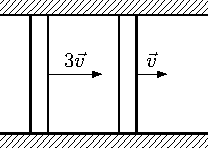
\includegraphics[width = 0.9 \textwidth]{0901LawOfConservationOfEnergyTwoPistons.jpg}
\end{minipage}
\begin{ans}
$T=T_0+2mv^2/3R$
\end{ans}
\end{ex}

%Черепанов
\begin{ex}
В длинной горизонтальной трубе могут скользить без трения два поршня, массы которых $m$ и $2m$. 
Между ними находится некоторое количество одноатомного газа при давлении $p$ и объеме $V$. 
В этот момент легкий поршень движется к тяжелому со скоростью $v_0$, тяжелый поршень покоится. 
Оцените максимальную скорость тяжелого поршня.
\begin{ans}
$v = v_0\left( 1 + \sqrt{1+9pV/2mv_0^2} \right)/3$
\end{ans}
\end{ex}

\begin{ex}
(2003) Внутри закрытого теплоизолированного цилиндра с идеальным газом находится легкоподвижный теплопроводящий поршень. 
При равновесии поршень делит цилиндр на две равные части и температура газа равна $T_0$. Поршень начали медленно перемещать. 
Найти температуру газа как функцию отношения $\eta$ объема большей части к объему меньшей части. Показатель адиабаты газа~$\gamma$.
\begin{ans}
$T=T_0 \left( (\eta + 1)^2/4 \eta \right)^{(\gamma-1)/2}$
\end{ans}
\end{ex}

\begin{ex}
\hspace{0pt} \\
\begin{minipage}{.65\textwidth}
Найдите КПД тепловой машины, цикл которой состоит из двух изохор и двух изобар, а рабочим телом является идеальный одноатомный газ. 
Середины нижней изобары и левой изохоры лежат на изотерме, соответствующей температуре $T_1$, 
а середины верхней изобары и правой изохоры -- на изотерме, соответствующей температуре~$T_2$.
\end{minipage}
\begin{minipage}{.35\textwidth}
\centering
\includestandalone{Pictures/0904LawOfConservationOfEnergyEfficiency}
\end{minipage}
\begin{ans}
$\eta = \frac{2(T_2-T_1)}{3T_1+5T_2}$
\end{ans}
\end{ex}

\begin{ex}
(2014) В вертикальном цилиндрическом сосуде с теплонепроницаемыми стенками под поршнем массы $m$~=~100~г находится 5 моль неона 
(молярная масса 20 г/моль). В начальный момент поршень закреплен. После того, как поршень освободили, объем газа увеличился в 2 раза. 
Определите конечную температуру газа, если его начальная температура равна $T_0$ = 300~К. Считайте, что над поршнем вакуум. 
Трением между поршнем и стенками сосуда отсутствует.
\begin{ans}
$T=2T_0/3 = 200$ К
\end{ans}
\end{ex}

\begin{ex}
(2015) B высоком теплоизолированном цилиндре под поршнем находится гелий. Над поршнем — вакуум. Поршню толчком сообщают скорость 2 м/с. На сколько выше или ниже начального положения окажется поршень после прихода системы в равновесие? Трением и теплообменом с внешней средой пренебречь.
\begin{ans}
$\Delta h = v_0^2 / 5g = 8$ см
\end{ans}
\end{ex}

\begin{ex}
(2016) B цилиндрическом сосуде с диэлектрическими стенками между металлическим основанием и металлическим поршнем находится двухтомный идеальный газ. Поршень и основание являются обкладками конденсатора, заряженного до напряжения $U$ и отключенного от источника питания, В равновесии расстояние между поршнем и основанием цилиндра равно $d$ (много меньше радиуса цилиндра) Площадь сечения сосуда равна $S$, слева от поршня - вакуум.
1) Определите отношение внутренней энергии газа и энергии электрического поля конденсатора. 2) Какое количество теплоты нужно сообщить газу для того, чтобы медленно увеличить расстояние между обкладками в 2 раза?
\begin{center}
\includestandalone{Pictures/GasInsideCapacitor}
\end{center}
\begin{ans}
1) $U/W=5/2$; 2) $Q=\frac{7\varepsilon_0 SU^2}{4d}$.
\end{ans}
\end{ex}

\begin{ex}
(2002) Чему равна работа 1 моля идеального газа в круговом процессе, показанном на рисунке? Температуры $T_1$ и $T_2$ известны.
\begin{center}
\includestandalone{Pictures/092002LawOfConservationOfEnergyProcess}
\end{center}
\begin{ans}
$A= R(T_2-T_1)-RT_1 \log T_2/T_1$
\end{ans}
\end{ex}

\begin{ex}
\hspace{0pt} \\
\begin{minipage}{.65\textwidth}
(2017) Идеальный одноатомный газ в количестве 0,1 моль находится под массивными поршнями в двух сообщающихся сосудах. Сосуды закрыты и откачаны, т.е. над поршнями вакуум. Массы поршней $m_1 = m_2 = 10$ кг, площади поперечного сечения поршней $S_1 = 10$ см\textsuperscript{2}, $S_2 = 20$ см\textsuperscript{2} B начальный момент времени первый поршень свободен, a второй — зафиксирован, поршни находятся на одинаковой высоте $h_1 = 80$ см. 1) Определите начальную температуру газа. 2) До какой температуры нагреется газ, если ему квазистатически сообщить тепло 100 Дж? 3) Определите температуру газа, которая установится, если в начальный момент времени сосуды теплоизолировать и освободить второй поршень. Трение отсутствует. Сосуды высокие, объемом очень тонкой перегородки, соединяющей сосуды, пренебречь. Ускорение свободного падения $g = 10$ м/c\textsuperscript{2}.
\end{minipage}
\begin{minipage}{.35\textwidth}
\centering
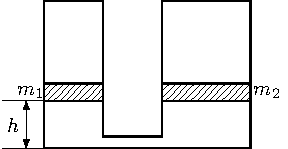
\includegraphics[width = 0.9 \textwidth]{TwoVessels.png}
\end{minipage}
\begin{ans}
1) $T_0 = m_1gh(1+S_2/S_1)/(\nu R) = 289$ К;
2) $T_2 = T_0 + 2Q/(5\nu R) = 337$ К; 
3) $T_3 = \frac{2}{5\nu R}(m_1 gh + m_2 gh)+ \frac{3}{5}T_0 = 250$ К.
\end{ans}
\end{ex}

\section{Теплоемкость}

\begin{ex}
(1998) Имеется идеальный газ, теплоемкость которого при постоянном объеме равна $C_V$. 
Найдите молярную теплоемкость этого газа как функцию объема, если давление газа меняется по закону $p=p_0~e^{\alpha V}$ ($p_0$ и $\alpha$ известны).
\begin{ans}
$C = C_V + R/(1+\alpha)$
\end{ans}
\end{ex}

%Черепанов
\begin{ex}
Для идеального газа с заданным показателем адиабаты $\gamma$ найдите уравнение процесса (в координатах $V$, $T$), при котором теплоемкость зависит от температуры по закону $C=\alpha T^2$.
\begin{ans}
$ V T^{1/(\gamma - 1)} = C e^{\alpha T^2 / 2R}$
\end{ans}
\end{ex}

\begin{ex}
\hspace{0pt} \\
\begin{minipage}{.65\textwidth}
(2005) В расположенном горизонтально цилиндре слева от закрепленного поршня находится один моль идеального газа, в правой части цилиндра - вакуум. Цилиндр теплоизолирован от окружающей среды, а пружина, расположенная между поршнем и стенкой, находится первоначально в недеформированном состоянии. Поршень освобождают, и после установления равновесия объем, занимаемый газом, увеличивается в $\alpha$ раз. Как изменились при этом температура и давление газа? Теплоемкостями цилиндра, поршня и пружины пренебречь. Найти теплоемкость газа.
\end{minipage}
\begin{minipage}{.35\textwidth}
\centering
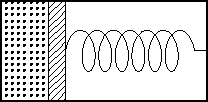
\includegraphics[width = 0.9 \textwidth]{092005HeatCapacityCylinder.jpg}
\end{minipage}
\begin{ans}
$T_2/T_1 = (\alpha i)/(\alpha (1+i) - 1)$, $p_2/p_1 = i/(\alpha (1+i) - 1)$
\end{ans}
\end{ex}

\begin{ex}
(2001) Вычислить молярную теплоемкость $C(V)$ идеального газа, совершающего процесс, показанный на рисунке. Показатель адиабаты $\gamma$ считать известным.
\begin{center}
\includestandalone{Pictures/082001GasLawsProcess}
\end{center}
\begin{ans}
$C(V) = R/(\gamma-1)+R(V_0-2V)/(V_0-2V)$
\end{ans}
\end{ex}

\chapter{Электричество}
\section{Электростатика}

\begin{ex}
Два маленьких шарика, массы которых $m$ и $M$, заряжены одинаковыми зарядами $q$ и удерживаются на расстоянии $L$ друг от друга. Шарики отпускают, и они начинают разлетаться. Найти скорости шариков после разлета на большое расстояние. Найти скорости шариков после разлета на расстояние $7L$.
\begin{ans}
$v = \sqrt{\frac{2Mq^2}{Lm(m+M)}}$, $u = \sqrt{\frac{2mq^2}{LM(m+M)}}$
\end{ans}
\end{ex}

%Ижевск
\begin{ex}
Точечный заряд $q$ находится между двумя заземленными проводящими концентрическими сферами 
радиусами $a$ и $b$ на расстоянии $r$ от центра ($a<r<b$). 
Найти полные индуцированные на сферах заряды. Рассмотреть все возможные предельные случаи.
\begin{ans}
$q_a = -q\frac{a(b-r)}{r(b-a)}$, $q_b = -q\frac{b(r-a)}{r(b-a)}$
\end{ans}
\end{ex}

%Ижевск
\begin{ex}
\hspace{0pt} \\
\begin{minipage}{.65\textwidth}
Заряженный металлический шар радиуса $R$ разрезан на две части по плоскости, отстоящей от центра на расстояние $h$. 
Найти силу, с которой отталкиваются эти части. Исходный заряд шара~$Q$.
\end{minipage}
\begin{minipage}{.35\textwidth}
\centering
\includestandalone{Pictures/1003ElectrostaticsBall}
\end{minipage}
\begin{ans}
$F = \frac{Q^2 \pi (R^2-h^2)}{2 \varepsilon_0 {(4 \pi R^2)}^2}$
\end{ans}
\end{ex}

%Ижевск
\begin{ex}
\hspace{0pt} \\
\begin{minipage}{.65\textwidth}
Грани правильного тетраэдра со стороной $a$ равномерно заряжены с поверхностной плотностью заряда $\sigma$. 
В центр тетраэдра помещен точечный заряд $q$. Найти силу, с которой точечный заряд действует на одну из граней тетраэдра.
\end{minipage}
\begin{minipage}{.35\textwidth}
\centering
\includestandalone{Pictures/1004ElectrostaticsTetrahedron}
\end{minipage}
\begin{ans}
$F = \frac{\sigma^2 \sqrt{3}a^2}{8\varepsilon_0}$
\end{ans}
\end{ex}

%Ижевск
\begin{ex}
\hspace{0pt} \\
\begin{minipage}{.65\textwidth}
Две большие проводящие пластины $1$ и $2$ расположены на расстоянии $d$ друг от друга, 
а между ними на расстоянии $x$ от пластины $1$ находится проводящая пластина с зарядом $q$. 
Крайние пластины соединены проводником и имеют заряд $-q$. 
Какой заряд пройдет по проводнику, соединяющему крайние пластины, если пластину с зарядом $q$ переместить из положения $x$ в положение с координатой~$x_1$.
\end{minipage}
\begin{minipage}{.35\textwidth}
\centering
\includestandalone{Pictures/1005ElectrostaticsTwoPlates}
\end{minipage}
\begin{ans}
$\mid\Delta q \mid = \mid q \frac{x-x_1}{d}$
\end{ans}
\end{ex}

\begin{ex}
(2017) В вакууме относительно некоторой ИСО покоится однородное тонкое кольцо радиуса $R$, массой $3m$ и равномерно распределенным зарядом $q$. Какую минимальную скорость в этой ИСО должна иметь частица массой $m$ и зарядом равным по знаку и величине заряду кольца, чтобы, двигаясь вдоль оси кольца с очень большого расстояния, достичь его центра? Рассмотрите два случая: а) кольцо закреплено; б) кольцо свободное.
\begin{ans}
$v_{\min} = q\sqrt{\frac{2k}{mR}}$, $v_{\min 2} = q\sqrt{\frac{8k}{3mR}}$, 
\end{ans}
\end{ex}

\section{Конденсаторы}

\begin{ex}
\hspace{0pt} \\
\begin{minipage}{.65\textwidth}
В электрической схеме, изображенной на рисунке, в начальный момент времени ключ $K$ разомкнут, конденсатор не заряжен. 
Параметры схемы указаны на рисунке. Определите начальные токи через резисторы и через батарею сразу после замыкания.
\end{minipage}
\begin{minipage}{.35\textwidth}
\centering
\includestandalone[width = 0.85 \textwidth]{Pictures/1001Condensers}
\end{minipage}
\begin{ans}
$I_{01} = \frac{3 \mathcal{E}}{3r+2R}$, $I_{02} = \frac{\mathcal{E}}{3r+2R}$
\end{ans}
\end{ex}

%Ижевск
\begin{ex}
\hspace{0pt} \\
\begin{minipage}{.65\textwidth}
Батарея с ЭДС, равной $\mathcal{E}$, конденсаторы емкостями $C_1$ и $C_2$ и резистор сопротивлением $R$ соединены так, как показано на рисунке. 
Найдите количество теплоты $Q$, выделяющееся на резисторе после переключения ключа~$K$.
\end{minipage}
\begin{minipage}{.35\textwidth}
\centering
\includestandalone[width = 0.85 \textwidth]{Pictures/1002Condensers}
\end{minipage}
\begin{ans}
$Q=\frac{C_1C_2 \mathcal{E}^2}{2(C_1+C_2)}$
\end{ans}
\end{ex}

\begin{ex} 
По какому закону изменяется ток через изначально незаряженный конденсатор емкости $C$, подключенный к источнику тока с напряжением $U$ через сопротивление $R$?
\begin{ans}
$I = \frac{U}{R} e^{-t/RC}$
\end{ans}
\end{ex}

\begin{ex} 
\hspace{0pt} \\
\begin{minipage}{.65\textwidth}
Две батареи включены в схему, изображенную на рисунке (сопротивления всех резисторов равны $R$). 
Первоначально конденсаторы не заряжены, а ключи разомкнуты. Ключи одновременно замыкают. 
1) Найти начальный ток через резистор $R_1$. 2) Какое количество теплоты выделится во всей схеме после замыкания ключей?
\end{minipage}
\begin{minipage}{.35\textwidth}
\centering
\includestandalone[width = 0.95\textwidth]{Pictures/1005Condensers}
\end{minipage}
\begin{ans}
1) $I_1=\frac{\mathcal{E}_1 + \mathcal{E}_2}{3R}$; 2) $Q=(C_1 \mathcal{E}_1^2 + C_2 \mathcal{E}_2^2/2)$
\end{ans}
\end{ex}

\begin{ex} 
\hspace{0pt} \\
\begin{minipage}{.65\textwidth}
В схеме на рисунке ключи разомкнуты, а конденсаторы не заряжены. Ключ $K_1$ замыкают, оставляя ключ $K_2$ разомкнутым. 
1) Какие напряжения установятся на конденсаторах? 2) Какой заряд протечет через ключ $K_2$ при замыкании?
\end{minipage}
\begin{minipage}{.35\textwidth}
\centering
\includestandalone[width = 0.85 \textwidth]{Pictures/1006Condensers}
\end{minipage}
\begin{ans}
1) $U_1 = \frac{2R \mathcal{E}}{r+3R}$, $U_2 = \frac{R \mathcal{E}}{r+3R}$; 2) $Q=\frac{3RC\mathcal{E}}{r+3R}$
\end{ans}
\end{ex}
\section{Постоянный электрический ток}

\begin{ex}
Найти сопротивления приведенных цепей между точками $A$ и $B$. Сопротивление каждого резистора известно и равно $R$.
\begin{center}
\includestandalone[scale=0.5]{Pictures/1101DirectCurrentABCircuitLine}
\includestandalone[scale=0.5]{Pictures/1101DirectCurrentABCircuitCube}
\includestandalone[scale=0.5]{Pictures/1101DirectCurrentABCircuitSquare}
\includestandalone[scale=0.5]{Pictures/1101DirectCurrentABCircuitStar}
\end{center}
\begin{ans}
$R/3$, $5R/6$, $6R/7$, $7R/15$
\end{ans}
\end{ex}

\begin{ex}
\hspace{0pt} \\
\begin{minipage}{.65\textwidth}
Сопротивления резисторов $R_1 = 1$ Ом, $R_2 = 2$ Ом, $R_3 = 3$ Ом, $R_4 =4$ Ом. 
Напряжение источника тока $U = 1$ В. Найдите ток, который течет через вертикальную перемычку.
\end{minipage}
\begin{minipage}{.35\textwidth}
\centering
\includestandalone[width = 0.8 \textwidth]{Pictures/1102DirectCurrentFourResistors}
\end{minipage}
\begin{ans}
$I = 2/21$ А
\end{ans}
\end{ex}

\begin{ex}
\hspace{0pt} \\
\begin{minipage}{.65\textwidth}
Три одинаковых медных кольца радиуса $r$ соединены так, как показано на рисунке. 
Найдите сопротивление полученной таким образом фигуры, внешнее напряжение подано к точкам $A$ и $B$. 
Удельное сопротивление меди $\rho$, диаметр проволоки~$d$.
\end{minipage}
\begin{minipage}{.35\textwidth}
\centering
\includestandalone[width = 0.75 \textwidth]{Pictures/1103DirectCurrentThreeRings}
\end{minipage}
\begin{ans}
$R = \rho r /16d^2$
\end{ans}
\end{ex}

\begin{ex}
Найдите эквивалентное сопротивление между точками $A$ и $B$ бесконечной цепочки, которая состоит из одинаковых резисторов сопротивлением $R$ каждый.

\centering
\includestandalone{Pictures/1104DirectCurrentFourInfiniteCircuitAB}
\begin{ans}
$(6-\sqrt{3})R/6$
\end{ans}
\end{ex}

\begin{ex}
\hspace{0pt} \\
\begin{minipage}{.65\textwidth}
Из бесконечной проводящей квадратной сетки, каждое звено которой имеет сопротивление $R$, удалили одно звено $AB$. Найдите сопротивление сетки между точками $A$ и $B$.
\end{minipage}
\begin{minipage}{.35\textwidth}
\centering
\includestandalone[scale = 0.7]{Pictures/1105DirectCurrentNet}
\end{minipage}
\begin{ans}
$R$
\end{ans}
\end{ex}

\begin{ex}
Имеется $n$ клемм, каждая из которых соединена со всеми остальными клеммами одинаковыми проводниками сопротивлением $R$. Найдите сопротивление между любыми двумя клеммами.
\begin{ans}
$R_1 = 2R/n$
\end{ans}
\end{ex}

\begin{ex}
Электрический чайник имеет две обмотки. При включении одной из них чайник вскипает через 10 мин, при включении другой -- через 15 мин. 
Через какое время чайник вскипит, если эти две обмотки включить вместе параллельно, последовательно?
\begin{ans}
$t_1 = 6$ мин, $t_2 = 25$ мин
\end{ans}
\end{ex}

\begin{ex}
\hspace{0pt} \\
\begin{minipage}{.65\textwidth}
На рисунке представлен график зависимости силы тока от напряжения на нелинейном резисторе. 
Определите силу тока в цепи при подключении этого резистора к источнику тока с напряжением 10 В и добавочным сопротивлением 100 Ом.
\end{minipage}
\begin{minipage}{.35\textwidth}
\centering
\includestandalone[width = 0.95 \textwidth]{Pictures/1108DirectCurrentVDR}
\end{minipage}
\begin{ans}
$I = 0,06$ А
\end{ans}
\end{ex}

\begin{ex}
\hspace{0pt} \\
\begin{minipage}{.65\textwidth}
На рисунке приведен график зависимости напряжения на разрядном промежутке дугового разряда от тока. Дугу подключают  к источнику постоянного напряжения последовательно с резистором. 
При каком максимальном значении сопротивления резистора дуга может гореть при напряжении источника $U =85$~В?
\end{minipage}
\begin{minipage}{.35\textwidth}
\centering
\includestandalone[width = 0.85 \textwidth]{Pictures/1109DirectCurrentArcDischarge}
\end{minipage}
\begin{ans}
$R = 5$ Ом
\end{ans}
\end{ex}

\begin{ex}
\hspace{0pt} \\
\begin{minipage}{.65\textwidth}
Схема, изображенная на рисунке, состоит из двух одинаковых резисторов $R_2$ и $R_3$ сопротивлением $R$ каждый и двух одинаковых нелинейных резисторов $R_1$ и $R_4$, вольтамперная характеристика которых имеет вид $U = \alpha I^2$. При каком напряжении источника питания $U_0$ сила тока через гальванометр равна нулю?
\end{minipage}
\begin{minipage}{.35\textwidth}
\centering
\includestandalone[width = 0.9 \textwidth]{Pictures/1110DirectCurrentResistorsAndGalvanometor}
\end{minipage}
\begin{ans}
$U_0 = 2R^2/\alpha$
\end{ans}
\end{ex}

\begin{ex}
(2018) Проволочный предохранитель перегорает при напряжении 300 В. При каком напряжении будет перегорать предохранитель, если его длину увеличить в 3 раза, a диаметр -- в 2 раза?
\begin{ans}
636 В
\end{ans}
\end{ex}
\section{Сила Ампера}

\begin{ex}
\hspace{0pt} \\
\begin{minipage}{.65\textwidth}
(2016) На рисунке представлена модель электродвигателя. Замкнутый контур образован двумя вертикальными рейками, между концами которых включен источник постоянного тока с ЭДС $\mathcal{E}$, a другие концы замкнуты перемычкой сопротивлением $R$ и длиной $L$. Перемычка за счет скользящих контактов может без трения скользить вдоль реек. Контур находится в однородном магнитном поле с индукцией $B$, направленной горизонтально. Известно, что если к перемычке подвесить груз массы $M$, она будет в состоянии равновесия. 1) Определите массу $m$ перемычки. 2) Определите установившуюся скорость ненагруженной перемычки. Сопротивлением реек и внутренним сопротивлением источника пренебречь.
\end{minipage}
\begin{minipage}{.35\textwidth}
\centering
\includestandalone{Pictures/RodInMagneticField}
\end{minipage}
\begin{ans}
1) $m=\mathcal{E}BL/Rg - M$; 2) $v = \frac{MgR}{B^2L^2}$
\end{ans}
\end{ex}

%Черепанов
\begin{ex}
(2003) Металлический стержень массой $m$ и длиной $L$ подвешен на двух легких проводах длиной $l$ в магнитном поле с индукцией $B$, 
вектор которой направлен вертикально. К точкам крепления проводов подключен конденсатор емкостью $C$, заряженный до напряжения $U$. 
Сопротивление стержня и проводов пренебрежимо мало. Найти максимальный угол отклонения проводов от вертикали, если разрядка конденсатора происходит за очень малое время.
\begin{ans}
$\sin \frac {\alpha}{2} = \frac{CUlB}{2m \sqrt{gL}}$
\end{ans}
\end{ex}

\begin{ex}
(2010) Посередине между двумя жестко закрепленными проводниками с током на расстоянии $a$ расположен груз массы $m$, представляющий собой цилиндрическую железную трубку длиной $l_1$ и укрепленный с помощью упругих растяжек длиной $l$. 
Магнитная проницаемость железа $\mu$. Внутри растяжек установлен еще один проводник. По всем трем проводникам течет ток $I$. 
Определите собственную частоту свободных колебаний груза, считая, что в процессе колебаний натяжение растяжек $T_0$ не изменяется. 
Определить зависимость критического значения силы тока от натяжения растяжек, считая критическим значением такое значение, при котором колебания в системе невозможны.
\begin{center}
\includestandalone{Pictures/122010AmperesForceLawTwoConductors}
\end{center}
\begin{ans}
$\omega^2 = \frac{2 T_0}{ml} - \frac{\mu \mu_0 I l_1}{\pi a^2}$, $I^* = \frac{2T_0 \pi a^2}{\mu \mu_0 l l_1}$
\end{ans}
\end{ex}

\begin{ex}
(2017) Одна из моделей генератора постоянного тока представляет собой проводящий диск, который вращается в однородном магнитном поле с индукцией,
направленной перпендикулярно плоскости вращения диска. Если концы некоторого проводника сопротивлением $R$ присоединить к центру диска и через скользящий контакт к его ободу, то в цепи возникнет электрический ток. 1) Объясните возникновение электрического тока и найдите силу тока, если радиус диска $r = 10$ см, частота вращения диска $\nu = 40$ об/с, индукция магнитного поля $B = 0,1$ Тл, сопротивление нагрузки $R = 0,5$ Ом. 2) Какая мощность затрачивается для поддержания вращения диска? 3) Какой момент силы относительно оси вращения нужно прикладывать к диску? Сопротивлениями диска и контактов пренебречь.
\begin{center}
\includestandalone{Pictures/AmperGenerator}
\end{center}
\begin{ans}
1) $I=\pi v B r^2/R = 251$ мА; 2) $P = I^2 R = 31,6$ мВт; 3) $M = P/2 \pi \nu = 126$ мкН м
\end{ans}
\end{ex}

\begin{ex}
\hspace{0pt} \\
\begin{minipage}{.65\textwidth}
(2009) Медная монета массой $m$ радиусом $R$ и толщиной $d$ движется в поле силы тяжести в однородном магнитном поле $B$. 
Вектор индукции магнитного поля направлен вдоль оси монеты и перпендикулярно ускорению свободного падения. Найти ускорение монеты.
\end{minipage}
\begin{minipage}{.35\textwidth}
\centering
\includestandalone[scale=0.9]{Pictures/122009EMICoin}
\end{minipage}
\begin{ans}
$a=g/(1+ \varepsilon_0 \pi R^2 d B^2 / m)$
\end{ans}
\end{ex}

\section{Закон Био-Савара-Лапласа}

%Иродов2.234
\begin{ex}
\hspace{0pt} \\
\begin{minipage}{.65\textwidth}
(1998) Ток $I$ течет по длинному прямому проводнику, сечение которого имеет форму тонкого полукольца радиуса $R$. Найти магнитную индукцию на оси~$O$.
\end{minipage}
\begin{minipage}{.35\textwidth}
\centering
\includestandalone{Pictures/HalfringMagn}
\end{minipage}
\begin{ans}
$B = \frac{\mu_0 I}{\pi^2 R}$
\end{ans}
\end{ex}

%Иродов2.265б
\begin{ex}
\hspace{0pt} \\
\begin{minipage}{.65\textwidth}
Найти модуль и направление силы, действующей на единицу длины тонкого проводника с током $I$ в точке $O$, если проводник изогнут так, как показано на рисунке.
\end{minipage}
\begin{minipage}{.35\textwidth}
\centering
\includestandalone{Pictures/1202BiotSavartLawConductor}
\end{minipage}
\begin{ans}
$F = \frac{\mu_0 I^2}{\pi l}$
\end{ans}
\end{ex}

\section{Теорема о циркуляции индукции магнитного поля}

%Ижевск
\begin{ex}
\hspace{0pt} \\
\begin{minipage}{.65\textwidth}
Однородный диэлектрический диск массой $m$ радиуса $R$, равномерно заряженный с полным зарядом $q$, помещен в однородное магнитное поле с индукцией $B$. Какую угловую скорость получит диск, если выключить магнитное поле?
\end{minipage}
\begin{minipage}{.35\textwidth}
\centering
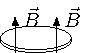
\includegraphics[width = 0.9 \textwidth]{1205AmperesCircuitalLawDisc.jpg}
\end{minipage}
\begin{ans}
$\omega = qB/2m$
\end{ans}
\end{ex}

%Ижевск
\begin{ex}
\hspace{0pt} \\
\begin{minipage}{.65\textwidth}
По поверхности жесткой непроводящей однородной сферы массой $m$ равномерно распределен заряд $q$. 
Сфера может свободно вращаться вокруг своей вертикальной оси. В начальный момент сфера покоилась, а магнитное поле было равно нулю. 
Найти, как меняется со временем угловая скорость сферы при включении однородного магнитного поля, 
сонаправленного с осью вращения сферы и меняющегося во времени по заданному закону $B(t)$.
\end{minipage}
\begin{minipage}{.35\textwidth}
\centering
\includegraphics[width = 0.9 \textwidth]{1206AmperesCircuitalLawSphere.jpg}
\end{minipage}
\begin{ans}
$\omega(t) = qB(t)/2m$
\end{ans}
\end{ex}
\section{Электромагнитная индукция}
%TODO Черепанов катушка + конденсатор + перемычка

\begin{ex}
\hspace{0pt} \\
\begin{minipage}{.65\textwidth}
(1998) По двум вертикальным рейкам, соединенным внизу сопротивлением $R$ и вверху источником с ЭДС $\mathcal{E}$ и внутренним сопротивлением $r$, без трения скользит проводник $AC$, длина которого $L$, масса $m$. 
Система находится в однородном магнитном поле с индукцией $B$, направленной за рисунок. 
Найдите установившуюся скорость проводника в поле силы тяжести, пренебрегая трением и сопротивлением реек и проводника.
\end{minipage}
\begin{minipage}{.35\textwidth}
\centering
\includestandalone{Pictures/121998EMIConductorAC}
\end{minipage}
\begin{ans}
$v = \frac{Rr}{lB(R+r)}\left( \frac{mg}{Bl} - \frac{\mathcal{E}}{r} \right)$
\end{ans}
\end{ex}

\begin{ex}
(2001) Две параллельные медные шины наклонены к горизонту под углом  $\alpha$. 
По ним скользит под действием силы тяжести медная перемычка массы $m$. Шины замкнуты катушкой с индуктивностью $L$. 
Система находится в однородном магнитном поле индукции $B$, перпендикулярном плоскости, в которой движется перемычка. 
Коэффициент трения перемычки о шины равен $\mu$. Каков будет характер движения перемычки? Сопротивлением шин, перемычки и катушки пренебречь.
\end{ex}

\begin{ex}
(2004) Металлический стержень массы $m$ и длины $L$ подвешен горизонтально на двух легких проводах длиной $h$ в магнитном поле, 
индукция которого $B$ направлена вертикально вниз. К точкам крепления проводов подключен конденсатор емкостью $C$. 
Стержень вывели из положения равновесия и отпустили. Определить период малых колебаний стержня $T$. Сопротивлением стержня и проводов пренебречь.
\begin{ans}
$T = 2\pi \sqrt{\frac{l}{g} \left( 1 + \frac{B^2L^2C}{ml} \right)}$
\end{ans}
\end{ex}

%Ижевск
\begin{ex}
По двум параллельным металлическим направляющим, наклоненным под углом $\alpha$ к горизонту и 
расположенным на расстоянии $l$ друг от друга, может скользить без трения металлическая перемычка массой $m$. 
Направляющие замкнуты снизу на незаряженный конденсатор емкостью $C$, и вся конструкция находится в магнитном поле, индукция которого $B$ направлена по вертикали. В начальный момент перемычку удерживают на расстоянии $l$ от основания "горки". 
Определите время $t$, за которое перемычка достигнет основания "горки"\ после того, как ее отпустят. 
Омическим сопротивлением и индуктивностью контура пренебречь.
\begin{center}
\includestandalone{Pictures/1211EMIHillAndBridge}
\end{center}
\begin{ans}
$t=\sqrt{\frac{2l}{g \sin \alpha} \left( 1 + \frac{C l^2B^2 \cos^2 \alpha}{m} \right)}$
\end{ans}
\end{ex}

%Иродов-2.325
\begin{samepage}
\begin{ex}
\hspace{0pt} \\
\begin{minipage}{.65\textwidth}
(2001) На расстоянии $a$ и $b$ от длинного прямого провода с током $I$ расположены два параллельных ему провода, 
замкнутые с одной стороны сопротивлением $R$. По проводам без трения перемещают с постоянной скоростью $v$ стержень-перемычку. 
Пренебрегая сопротивлением проводов, стержня и контактов, найдите силу, необходимую для поддержания постоянства скорости. 
На каком расстоянии от ближнего провода нужно приложить силу, чтобы избежать вращения стержня?
\end{minipage}
\begin{minipage}{.35\textwidth}
\centering
\includestandalone[width = 0.8 \textwidth]{Pictures/122001EMIWiresAndBar}
\end{minipage}
\begin{ans}
$F=\frac{\mu_0^2 I^2 v}{4 \pi^2 R} \log^2 \frac{b}{a}$
\end{ans}
\end{ex}
\end{samepage}

%Ижевск
\begin{ex}
\hspace{0pt} \\
\begin{minipage}{.65\textwidth}
(2002) Прямоугольная рамка со сторонами $a$ и $b$ находится в одной плоскости с прямым проводником, по которому течет ток $I$, на расстоянии $L$ от него. Какой импульс получит рамка при выключении тока в проводе, если активное сопротивление рамки равно $R$, а реактивным сопротивлением ее можно пренебречь? 
Считать, что за время передачи импульса рамка заметно не перемещается.
\end{minipage}
\begin{minipage}{.35\textwidth}
\centering
\includestandalone[width = 0.8 \textwidth]{Pictures/122002EMIFrame}
\end{minipage}
\begin{ans}
$p=\frac{\mu_0^2ab^2I^2}{8\pi^2RL(L+a)}\log\left( 1+\frac{a}{L} \right)$
\end{ans}
\end{ex}

% Московская олимпиада школьников
\begin{ex}
Параллельные рельсы длиной $2L$ закреплены на горизонтальной плоскости на расстоянии $l$ друг от друга. 
К их концам подсоединены две одинаковые батареи с ЭДС  $\mathcal{E}$. На рельсах лежит перемычка массы $m$, 
которая может поступательно скользить вдоль них. Вся система помещена в однородное вертикальное магнитное поле с индукцией $B$. 
Считая, что сопротивление перемычки равно $R$, а сопротивление единицы длины каждого из рельсов равно $\rho$, найдите период малых колебаний, возникающих при смещении перемычки от положения равновесия, пренебрегая затуханием, внутренним сопротивлением источников, сопротивлением контактов, а также индуктивностью цепи.
\begin{center}
\includestandalone{Pictures/1214EMIRailsAndBridge}
\end{center}
\begin{ans}
$T_0 = 2 \pi \sqrt{\frac{mL(\rho L + R)}{\mathcal{E}lB}}$
\end{ans}
\end{ex}

\begin{ex}
(2015) Проводящая квадратная рамка пересекает область однородного магнитного поля с шириной $d$, линии напряженности которого перпендикулярны плоскости рамки. При этом скорость рамки, равная $v_0$ до входа в магнитное поле уменьшается в 2 раза. Масса рамки равна $m$, сопротивление рамки $R$, величина вектора магнитной индукции $B$. 1) Объясните, почему в рамке при пересечении магнитного поля выделяется тепло и найдите его. 2) Определите длину стороны рамки $a$ предполагая, что $a<d$. 3) Определите длину стороны рамки $a$ предполагая, что $a>d$.
\begin{ans}
1) $Q = 3mv_0^2/8$; 2) $a=\sqrt[3]{\frac{mv_0R}{4B^2}}$; 3) $a=\sqrt{\frac{mv_0R}{4B^2d}}$
\end{ans}
\end{ex}
\section{Движение заряженных частиц}

\begin{ex}
Заряженная частица массы $m$ зарядом $q$ влетает в магнитное поле $B$ под углом $\alpha$ со скоростью $v$. По какой траектории движется частица? Каков пространственный период витка (шаг спирали)?
\begin{ans}
$d = 2 \pi v \cos \alpha m / qB$
\end{ans}
\end{ex}

%Ижевск
\begin{ex}
По обмотке длинного цилиндрического соленоида радиуса $R$ протекает постоянный ток, создающий внутри соленоида однородное магнитное поле с индукцией $B$. Между витками соленоида в него влетает по радиусу (перпендикулярно оси соленоида) электрон со скоростью $v$. Отклоняясь в магнитном поле, электрон спустя некоторое время покинул соленоид. Определите время движения внутри соленоида.
\begin{ans}
$t=\frac{2m}{eB}\arctan \left( \frac{eBR}{mv}\right)$
\end{ans}
\end{ex}

\begin{ex}
\hspace{0pt} \\
\begin{minipage}{.65\textwidth}
(2018) Вакуумный диод представляет собой две металлические пластины -- катод и анод. Между пластинами имеется однородное магнитное поле с индукцией $B$, параллельной плоскости пластин (направленной из плоскости чертежа). Расстояние между пластинами $d$. Из катода вылетают электроны. 1) При каких начальных скоростях все электроны не смогут достичь анода при $U = 0$? 2) При каких напряжениях $U$ все электроны не смогут достичь анода при нулевой начальной скорости?
\end{minipage}
\begin{minipage}{.35\textwidth}
\centering
\includestandalone{Pictures/ElectronInVacuumDiode}
\end{minipage}
\begin{ans}
1) $v_0 < eBd/m$; 2) $U < eB^2d^2/2m$
\end{ans}
\end{ex}

\begin{ex}
(2014) Незаряженная неподвижная частица распалась в однородном магнитном поле с индукцией $B$ на две частицы с массами $m_1$ и $m_2$ и зарядами $+q$ и $-q$. Найдите время, через которое произойдет соударение частиц. Кулоновским взаимодействием между частицами пренебречь.
\begin{ans}
$t = \frac{2\pi m_1 m_2}{qB(m_1+m_2)}$
\end{ans}
\end{ex}

\begin{ex}
(2008) Электронно-лучевая трубка помещена в однородное магнитное поле, напряженность $H$ которого перпендикулярна плоскости экрана. Электроны влетают в электронно-лучевую трубку из электронной пушки с составляющей скорости $u$ вдоль оси трубки и составляющей скорости $v_0$ перпендикулярно оси. При какой длине $L$ трубки все электроны фокусируются в одной точке экрана?
\begin{ans}
$L=2\pi m u n/ eB$, $n \in \mathcal{N}$
\end{ans}
\end{ex}

\begin{ex}
(2012) Две заряженные частицы движутся в однородном магнитном поле $B$, причем $q_1/m_1 = q_2/m_2$. Написать уравнения движения центра масс и уравнение относительного движения.
\begin{ans}
$\vec{a}_c = \frac{q_1}{m_1}\vec{v}_c \times \vec B$, 
${\vec{r}}^{\prime \prime} = \frac{q_1}{m_1}\vec{r}^{\prime} \times \vec B + \frac{q_1(q_2-q_1)\vec r}{m_1 r^3}$
\end{ans}
\end{ex}

\begin{ex}
(2013) Заряд $q$ движется в поле магнитного монополя $\vec{B} = \alpha \vec{r}/r^3$. Найдите интеграл движения, следующий из закона изменения момента импульса заряда.
\begin{ans}
$\vec r \times \vec p - \alpha q \vec r/ r = \text{const} $
\end{ans}
\end{ex}

\begin{ex}
Частица c зарядом $q$ и массой $m$ движется с начальной скоростью $v_0$ в вязкой среде в поперечном магнитном поле с индукцией $B$. Сила сопротивления $\vec{F} = -\gamma \vec{v}$, где $\gamma$ - константа. На каком расстоянии от начальной точки частица остановится?
\begin{sol}
На частицу действуют сила вязкого трения $\vec{F} = - r\vec{v}$ и сила Лоренца $\vec{F_L} = q \vec{v} \times \vec{B}$, уравнение движения в проекциях на оси, перпендикулярные $\vec{B}$, имеет вид:  $m \dot{v_x}=-rv_x+q v_y B$, $m \dot{v_y}=-rv_y-q v_x B$. Умножим второе из этих уравнений на $i$ и сложим с первым, получим $m\left( \dot{v_x} +i \dot{v_y} \right) = -r(v_x+i v_y) - iqB(v_x+i v_y)$. Обозначим $\phi \equiv v_x+i v_y$, тогда получим для $\phi$ дифференциальное уравнение $\dot{\phi} + \delta \phi + i\omega \phi=0$, где $\delta=r/m$,  $\omega=qB/m$. Решение этого уравнения, удовлетворяющее начальным условиям $v_x(0)=v_0$, $v_y(0)=0$, имеет вид $\phi(t)=v_0 e^{-(\delta +i\omega) t}$. Расстояние от начальной точки до точки, где частица остановится, $L=\sqrt{x_{\infty}^2 + y_{\infty}^2} =\sqrt{ \left( \int_{0}^{\infty}{v_x \, dt} \right)^2 + \left( \int_{0}^{\infty}{v_y \, dt} \right)^2}=\vert \int_{0}^{\infty}{ \phi \, dt} \vert=v_0/\sqrt{\delta^2 +\omega^2}=m v_0/\sqrt{r^2+q^2B^2}$.
\end{sol}
\begin{ans}
$r_{\infty} = mv_0/\sqrt{\gamma^2 + q^2B^2}$
\end{ans}
\end{ex}

\begin{ex}
(2007) Частица c зарядом $q$ и массой $m$ движется в постоянных однородных скрещенных полях $\vec{E} \bot \vec{H}$ в среде с малым линейным сопротивлением $\vec{F} = -\gamma \vec{v}$. Найти скорость частицы вдоль поля $\vec{E}$, усредненную по периоду.
\begin{ans}
$\langle v \rangle = \frac{E}{B}\left(\frac{\beta}{2\omega} + 2\pi \frac{\beta^2}{\omega^2} \right)$, $\beta = 2\gamma/m$, $\omega = \sqrt{\frac{q^2B^2+\gamma^2}{m^2}} \approx \frac{qB}{m}$
\end{ans}
\end{ex}

%Ижевск, Черепанов
\begin{ex}
На магнитный барьер, задаваемый в пространстве статическим магнитным полем $\vec{B} = \left(0, 0, \frac{B_0}{\cosh^2(ky)}\right)$, где $k$ -- константа, из бесконечности налетает протон с начальной скоростью $\vec{v}_{-\infty} = (0, v_0, 0)$, $\vec{r}_{-\infty} = (0, -\infty, 0)$. Оцените минимальную скорость, которую должен иметь протон, чтобы преодолеть барьер и уйти на бесконечность. 
\begin{ans}
$v_0 = 2qB_0/(mk)$
\end{ans}
\end{ex}

%Черепанов
\begin{ex}
(2005)  Магнетрон -- это прибор, состоящий из нити накала радиуса $a$ и коаксиального цилиндрического анода радиуса $b$, которые находятся в однородном магнитном поле параллельном нити. Между нитью и анодом приложена ускоряющая разность потенциалов $U$. Найти минимальное значение индукции магнитного поля $B$, при котором электроны, вылетающие с нулевой начальной скоростью из нити, не будут достигать анода.
\begin{ans}
$B=\frac{b}{b^2-a^2}\sqrt{\frac{8mU}{e}}$
\end{ans}
\end{ex}

\chapter{Колебания}
\section{Механические колебания}
%TODO разделы
%TODO задача краевой олимпиады 2007


%-----------------Пружинный маятник---------------------
%Ландау
\begin{ex}
\hspace{0pt} \\
\begin{minipage}{.65\textwidth}
Найдите частоту колебаний точки с массой $m$, способной двигаться по прямой и прикрепленной к пружине, другой конец которой закреплен в точке $A$ на расстоянии $l$ от прямой. Пружина, имея длину $l$, натянута с силой $F$.
\end{minipage}
\begin{minipage}{.35\textwidth}
\centering
\includestandalone[width = 0.95 \textwidth]{Pictures/1303OscillationsSpringAndLine}
\end{minipage}
\begin{ans}
$\omega = \sqrt{F/ml}$
\end{ans}
\end{ex}

%Ландау
\begin{ex}
\hspace{0pt} \\
\begin{minipage}{.65\textwidth}
Найдите частоту колебаний точки с массой $m$, способной двигаться по окружности радиуса $r$ и прикрепленной к пружине, другой конец которой закреплен в точке $A$, кратчайшее расстоянии то точки $A$ до окружности равно $l$. Пружина, имея длину $l$, натянута с силой $F$.
\end{minipage}
\begin{minipage}{.35\textwidth}
\centering
\includestandalone[width = 0.95 \textwidth]{Pictures/1304OscillationsSpringAndCircle}
\end{minipage}
\begin{ans}
$\omega = \sqrt{\frac{F(r+l)}{rml}}$
\end{ans}
\end{ex}

\begin{ex}
\hspace{0pt} \\
\begin{minipage}{.65\textwidth} 
(2007) С какой частотой $\omega_0$ будет совершать малые вертикальные колебания в поле тяжести груз массы $m$, подвешенный на двух одинаковых пружинах жесткости $k$, образующих в равновесии углы $\beta$ с вертикалью?
\end{minipage}
\begin{minipage}{.35\textwidth}
\centering
\includestandalone[width = 0.95 \textwidth]{Pictures/132007OscillationsTwoSpringsAndWeight}
\end{minipage}
\begin{ans}
$\omega = \cos \beta \sqrt{2k/m}$
\end{ans}
\end{ex}

%Иродов-3.51
\begin{ex}
\hspace{0pt} \\
\begin{minipage}{.65\textwidth} 
Найти круговую частоту малых колебаний тонкого стержня массы $m$ и длины $l$ вокруг горизонтальной оси, проходящей через точку $O$. 
Жесткость пружины $k$. В положении равновесия стержень вертикален.
\end{minipage}
\begin{minipage}{.35\textwidth}
\centering
\includestandalone{Pictures/SpringRodOsc}
\end{minipage}
\begin{ans}
$\omega = \sqrt{3g/2l+3k/m}$
\end{ans}
\end{ex}

\begin{ex}
(2016) Студент университета Пружинкин, увлекающийся физическим экспериментом (и не очень любящий теорию) смонтировал в физической лаборатории маятник. Маятник представлял собой очень легкий шарнирно закрепленный стержень длины $l = 50$ см (шарнир в нижней точке стержня), на котором были закреплены два одинаковых шарика c массами по $m = 0,9$ кг: один шарик -- в середине стержня, a другой нa верхнем его конце. Между стержнем и вертикальной неподвижной стенкой на высоте $h=3l/4$ от шарнира студент закрепил горизонтальные пружинки различной жесткости. В положении равновесия деформация пружинок была равна нулю. Для того, чтобы построить экспериментальный график зависимости периода малых колебаний от жесткости, студент изготовил для опытов пять пружинок с известными жесткостями $k = 10, 20, 30, 40, 50$ Н/м. Выведите выражение для периода колебаний маятника и предскажите результаты опытов Пружинкина.
\begin{center}
\includestandalone{Pictures/InvertedPenduumWithSpring}
\end{center}
\begin{ans}
$T=2\pi \sqrt{\frac{20ml}{9kl-24mg}}$, при $k>24mg/9l$
\end{ans}
\end{ex}

\begin{ex}
(2015) На гладкой горизонтальной поверхности находится грузик, прикрепленный двумя одинаковыми пружинами к стенкам (вид сверху на рисунке слева). 
В положении равновесии грузика пружины имеют одинаковое растяжение~$\Delta l$. 1) В первом случае груз совершает малые колебания вдоль оси~$x$. 
Как зависит период этих колебаний от величины~$\Delta l$?   2) Во втором случае траектория грузика, совершающего малые колебания, изображена на рисунке справа (в увеличенном виде).
Определите $\Delta l$, если длина пружин в нерастянутом состоянии $l$~=~15 см. Во всех случаях выполняется закон Гука.
\begin{center}
\includestandalone{Pictures/132015OscillationsLissajousCurve}
\end{center}
\begin{ans}
$\omega_x = \sqrt{2k/m}$, $\omega_y=\sqrt{\frac{2k\Delta l}{m(l+\Delta l)}}$, $\Delta l = l/3$
\end{ans}
\end{ex}

%Ижевск
\begin{ex}
\hspace{0pt} \\
\begin{minipage}{.65\textwidth}
Схема динамического поглотителя колебаний представлена на рисунке. На первую массу действует гармоническая сила $F(t)~=~F_0\,\sin\,\omega\,t$. 
При каких условиях амплитуда вынужденных колебаний первой массы будет равна нулю?
\end{minipage}
\begin{minipage}{.35\textwidth}
\centering
\includestandalone{Pictures/1302OscillationsDynamicAbsorbentOfOscillations}
\end{minipage}
\begin{ans}
$\omega = \sqrt{k_2/m_2}$
\end{ans}
\end{ex}

%Черепанов
\begin{ex}
Груз массой $m$ прикреплен к пружине жесткостью $k$, а пружина к точке подвеса. 
Под действием внешней силы точка подвеса колеблется в вертикальном направлении по закону $x_p~=~A~\cos\,\omega t$. 
Какова амплитуда установившихся колебаний груза в вязкой среде, если сила сопротивления пропорциональна скорости $(F~=~-bv)$?
\begin{ans}
$x^2 = A^2\frac{\omega_0^4+4\beta^2\omega^2}{(\omega_0^2-\omega^2)^2+4\beta^2\omega^2}$, $\omega_0 = \sqrt{k/m}$, $\beta = b/2m$
\end{ans}
\end{ex}

%-------------Колебания газа в банке---------------
%Бутиков
\begin{ex} Расположенный горизонтально цилиндрический сосуд объема $V$, заполненный $\nu$ молями идеального газа, 
разделен поршнем массы $m$, который может двигаться без трения. В равновесии поршень находится посередине цилиндра. 
При малых смещениях из положения равновесия поршень совершает колебания. Найдите зависимость частоты этих колебаний от температуры, 
считая процесс изотермическим. Площадь поперечного сечения трубки равна~$S$.
\begin{ans}
$\omega^2=\frac{2\nu R S^2}{mV^2}T$
\end{ans}
\end{ex}

%Ижевск
\begin{ex}
\hspace{0pt} \\
\begin{minipage}{.65\textwidth} 
В длинной вертикальной цилиндрической трубке, закрытой с нижнего конца, может ходить без трения поршень, 
масса $M$ которого велика по сравнению с массой газа, заключенного внутри трубки. В положении равновесия расстояние между поршнем и дном трубки равно $L$. 
Определить период малых колебаний, которые возникнут при отклонении поршня от положения равновесия, в предположении, что они являются изотермическими, 
а газ идеальным. Площадь поперечного сечения трубки равна $S$, атмосферное давление равно $p_0$. Рассмотреть предельный случай, когда $p_0$~=~0.
\end{minipage}
\begin{minipage}{.35\textwidth}
\centering
\includestandalone{Pictures/1308OscillationsPistonInVerticalTube}
\end{minipage}
\begin{ans}
$T=2\pi\sqrt{\frac{ML}{p_0S + Mg}}$
\end{ans}
\end{ex}

%-----------Колебания жидкости-------------
%Иродов-3.20
\begin{ex}
\hspace{0pt} \\
\begin{minipage}{.65\textwidth} 
Идеальная жидкость объема $V$ налита в изогнутую трубку с площадью сечения канала $S$. Найти период малых колебаний жидкости.
\end{minipage}
\begin{minipage}{.35\textwidth}
\centering
\includestandalone{Pictures/1310OscillationsPerfectLiquid}
\end{minipage}
\begin{ans}
$T=\pi \sqrt{2V/Sg}$
\end{ans}
\end{ex}

%Иродов-3.21
\begin{ex}
Трубка высотой $H$ наполнена жидкостью и соединена с наклонной трубкой (угол наклона к вертикали $\alpha$). Каков будет период колебаний жидкости в такой системе?
\begin{ans}
$T=2\pi \sqrt{H/g(1+\cos \alpha)}$
\end{ans}
\end{ex}

\begin{ex}
\hspace{0pt} \\
\begin{minipage}{.65\textwidth} 
(2006) В тонкой трубке может скользить без трения веревка длиной $L$. В начальный момент времени веревка находится в левом колене. 
Определить период колебаний $T$ веревки. Жесткостью веревки на изгиб пренебречь. 
Каким будет период колебаний $T_1$, если расстояние между вертикальными коленами трубки увеличить с $L$ до $2L$?
\end{minipage}
\begin{minipage}{.35\textwidth}
\centering
\includestandalone{Pictures/132006OscillationsRopeInTube}
\end{minipage}
\begin{ans}
$T=2\pi\sqrt{L/g}$, $T=2(\pi+1)\sqrt{L/g}$
\end{ans}
\end{ex}

%-----------Затухающие колебания-------------

% Иродов-3.88
\begin{ex}
\hspace{0pt} \\
\begin{minipage}{.65\textwidth} 
Тонкий однородный диск массы $m$ и радиуса $R$, подвешенный в горизонтальном положении к упругой нити, совершает крутильные колебания в жидкости. 
Момент упругих сил со стороны нити $M~=~\alpha\,\varphi$.  Сила сопротивления на единицу поверхности $F~=~\eta\,v$. Найти частоту малых колебаний.
\end{minipage}
\begin{minipage}{.35\textwidth}
\centering
\includestandalone{Pictures/1309OscillationsDisc}
\end{minipage}
\begin{ans}
$\omega = \sqrt{2\alpha/mR^2-(\pi \eta R^2/m)^2}$
\end{ans}
\end{ex}

%Черепанов
\begin{ex}
(2004) На горизонтальной плоскости с коэффициентом трения $\mu$ лежит брусок массы $m$, который пружиной жесткости $k$ соединен с вертикальной стенкой. Брусок сместили на расстояние $9\mu mg /2k$ и отпустили. Найти число колебаний бруска до остановки.
\begin{ans}
одно колебание
\end{ans}
\end{ex}

%------------Колебания в поле силы тяжести------------
\begin{ex}
\hspace{0pt} \\
\begin{minipage}{.65\textwidth} 
Найти период малых колебаний плоского маятника, точка подвеса которого с массой $M$ находится на гладкой горизонтальной прямой 
(масса маятника $m$ и его длина $L$).
\end{minipage}
\begin{minipage}{.35\textwidth}
\centering
\includestandalone{Pictures/1314OscillationsPlanePendulum}
\end{minipage}
\begin{ans}
$T=2\pi \sqrt{\frac{L}{g(1+m/M)}}$
\end{ans}
\end{ex}

%Ижевск
\begin{ex}
Дана проволочная вешалка, которая качается с малой амплитудой в плоскости рисунка относительно заданных положений равновесия. 
В положениях а и б длинная сторона вешалки расположена горизонтально. Две другие стороны равны между собой. 
Во всех трех случаях (а, б, в) возникают колебания с одинаковыми периодами. Где расположен центр масс вешалки?
\begin{center}
\includestandalone{Pictures/1315OscillationsHanger}
\end{center}
\begin{ans}
На расстоянии 5 см от вершины треугольника
\end{ans}
\end{ex}

\begin{ex}
\hspace{0pt} \\
\begin{minipage}{.65\textwidth}
(2013) Точка подвеса математического маятника движется с постоянным ускорением $a$ (лежащим в плоскости колебаний маятника) в горизонтальном направлении. Найти закон движения маятника.
\end{minipage}
\begin{minipage}{.35\textwidth}
\centering
\includestandalone{Pictures/132013OscillationsMathematicalPendulum}
\end{minipage}
\begin{ans}
$\alpha(t) = A \cos(\sqrt{\sqrt{a^2+g^2}/l}t) + \alpha_0$, $\alpha_0 = \arctan(a/g)$
\end{ans}
\end{ex}

\begin{ex}
(2017) Один конец однородного стержня длиной $L=1$ м закреплен на горизонтальной оси $O$ (перпендикулярной плоскости чертежа), вокруг которой он может вращаться без трения. Другой конец стержня свободно лежит на опоре $A$, при этом стержень горизонтали. Свободный конец стержня приподнимают на высоту $h = 1$ см относительно исходного положения, поворачивая стержень
вокруг оси $O$, и отпускают бы начальной скорости. 1) Определите скорость
свободного конца стержня при ударе об опору $A$. 2) Определите частоту ударов
стержня об опору $A$, считая удары абсолютно упругими и мгновенными.
Ускорение свободного падения $g$ = 10 м/с\textsuperscript{2}. Трением пренебречь.
\begin{center}
\includestandalone{Pictures/HittingRod}
\end{center}
\begin{ans}
1) $v=\sqrt{3gh}$; 2) $\nu = 0.25\sqrt{3g/h }$
\end{ans}
\end{ex}

\begin{ex}
(2010) На абсолютно гибкой нити подвешен маятник. Расстояния до точки подвеса равны $S_1$ и $S_2$. 
Статический прогиб в точке подвеса маятника равен $y_0$, а длина маятника $l$, его масса $m$. 
Принять, что при $t$~=~0 точка подвеса имеет вертикальное смещение $A$, а ее скорость $v_0$ равна нулю; маятник отклонен на угол $\varphi_0$. 
Считая, что натяжение нити $T = T_0 = \text{const}$, вывести дифференциальное уравнение малых колебаний маятника.
\begin{center}
\includestandalone{Pictures/132010OscillationsPendulumOnThread}
\end{center}
\begin{ans}
$ml \varphi^{\prime \prime} + (mg-m \omega^2 A \cos \omega t) \varphi = 0$, $\omega^2 = T_0(S_1+S_2)/m S_1 S_2$
\end{ans}
\end{ex}

\begin{ex}
(2014) В центре плоского конденсатора удерживают диполь в положении 1, указанном на рисунке. 
Диполь представляет собой два маленьких заряженных шарика с зарядами $q$ и $-q$ и массами $m$ каждый, 
соединенных невесомым непроводящим стержнем длины $L$. Разность потенциалов между пластинами конденсатора равна $U$, 
расстояние между пластинами равно $d$ (много меньше размеров пластин). Диполь поворачивают вокруг его центра и переводят в положение 2, 
которое является устойчивым положением равновесия диполя. 
1) Определите работу электрического поля при повороте диполя из положения 1 в положение 2. 
2) Определите период малых крутильных колебаний диполя вокруг положения 2. 
3) Какую минимальную скорость нужно сообщить диполю в положении 2 параллельно пластинам для того, чтобы диполь улетел из конденсатора? 
Силу тяжести не учитывать.
\begin{center}
\includestandalone{Pictures/132014OscillationsCondenserAndDoublet}
\end{center}
\begin{ans}
1) $A=qUL/d$; 2) $T=2\pi\sqrt{\frac{mLd}{2qU}}$; 3) $v_0 = \sqrt{\frac{qUL}{md }}$
\end{ans}
\end{ex}

\begin{ex}
Молекулу одноатомного газа массы $m$, совершающую колебания около некоторого положения равновесия с амплитудой $a$ и частотой $\omega$, 
в первом приближении можно считать линейным гармоническим осциллятором. 
Найти $f(x)$ -- функцию распределения вероятностей значений координаты $x$ такого осциллятора, среднее значение координаты $\langle x \rangle$, 
среднее значение $\langle U \rangle$ потенциальной энергии осциллятора.
\end{ex}
\section{Колебательный контур}

%Ижевск
\begin{ex}
\hspace{0pt} \\
\begin{minipage}{.65\textwidth}
Батарея из двух последовательных соединенных конденсаторов емкостью $C$ каждый заряжена до напряжения $U$ и в начальный момент времени подключена к катушке индуктивностью $L$, так что образовался колебательный контур. 
Спустя интервал времени $\tau$ один из конденсаторов пробивается, и сопротивление между обкладками становится равным нулю. 
Найдите амплитуду колебаний заряда на непробитом конденсаторе.
\end{minipage}
\begin{minipage}{.35\textwidth}
\centering
\includestandalone{Pictures/1219OscillatoryCircuitCCL}
\end{minipage}
\begin{ans}
$q_{\max} = \frac{CU}{2}\sqrt{2-\cos^2 \left( \sqrt{\frac{2}{LC}} \tau \right)}$
\end{ans}
\end{ex}

%Кабардин-12.4
\begin{ex}
\hspace{0pt} \\
\begin{minipage}{.65\textwidth}
 Два конденсатора одинаковой электроемкости $C_1 = C_2 = C$ и катушка индуктивности $L$ соединены так, как показано на рисунке. 
В начальный момент времени ключ разомкнут, конденсатор $C_1$ заряжен до разности потенциалов $U$, а конденсатор $C_2$ не заряжен, 
сила тока в катушке равна нулю. Определите максимальное значение силы тока в катушке после замыкания цепи и период электромагнитных колебаний в цепи. 
\end{minipage}
\begin{minipage}{.35\textwidth}
\centering
\includestandalone{Pictures/1220OscillatoryCircuitC1C2L}
\end{minipage}
\begin{ans}
$I_{\max} = U \sqrt{\frac{C}{2L}}$, $T=2 \pi \sqrt{2LC}$
\end{ans}
\end{ex}

%Ижевск
\begin{ex}
\hspace{0pt} \\
\begin{minipage}{.65\textwidth}
В схеме, изображенной на рисунке, в некоторый момент времени замыкают ключ $K$, и конденсатор емкостью $C$, имеющий первоначальный заряд $q_0$, начинает заряжаться через катушку индуктивности $L$. 
Когда ток разряда достигает максимального значения, ключ $K$ вновь размыкают. Найти заряд $Q$, который протечет через резистор $R$. 
Сопротивление диода в прямом направлении много меньше $R$, в обратном -- бесконечно велико.
\end{minipage}
\begin{minipage}{.35\textwidth}
\centering
\includestandalone{Pictures/1221OscillatoryCircuitCLR}
\end{minipage}
\begin{ans}
$q=\frac{q_0}{R}\sqrt{\frac{L}{C}}$
\end{ans}
\end{ex}

\begin{ex}
\hspace{0pt} \\
\begin{minipage}{.65\textwidth}
(2011) Электрический контур представляет собой треугольник, каждая сторона которого содержит емкость $C$, а вершины соединены с общей центральной точкой индуктивностями $L$. 
Пренебрегая сопротивлением и взаимной индуктивностью, найдите частоту возможных колебаний.
\end{minipage}
\begin{minipage}{.35\textwidth}
\centering
\includestandalone[width = 0.95\textwidth]{Pictures/122011OscillatoryCircuitTriangleCCCLLL}
\end{minipage}
\begin{ans}
$\omega = 1/\sqrt{3LC}$
\end{ans}
\end{ex}

\section{Переменный электрический ток}

%Ижевск
\begin{ex}
\hspace{0pt} \\
\begin{minipage}{.65\textwidth}
В изображенной на рисунке электрической цепи определите частоту приложенного переменного напряжения, при которой переменный ток через сопротивление не зависит от значения $R$. Индуктивность $L$ и емкость $C$ считать известными.
\end{minipage}
\begin{minipage}{.35\textwidth}
\centering
\includestandalone{Pictures/1223AlternatingCurrentCLR}
\end{minipage}
\begin{ans}
$\omega = 1/\sqrt{LC}$
\end{ans}
\end{ex}

%Козел-10.5
\begin{ex}
\hspace{0pt} \\
\begin{minipage}{.65\textwidth}
В приведенной на рисунке схеме в момент $t$~=~0 замыкают ключ $K$. Найти зависимость от времени тока $I$, текущего через источник синусоидальной ЭДС $\mathcal{E}~=~\mathcal{E}_0 \sin \omega t$.
Параметры контура связаны соотношением $R\,=\,\sqrt{L/C}$.
\end{minipage}
\begin{minipage}{.35\textwidth}
\centering
\includestandalone[width = 0.95 \textwidth]{Pictures/1225AlternatingCurrentCLRR}
\end{minipage}
\begin{ans}
$I(t) = \frac{\mathcal{E}_0}{R} \sin \omega t$
\end{ans}
\end{ex}

%Козел-10.52
\begin{samepage}
\begin{ex}
\hspace{0pt} \\
\begin{minipage}{.65\textwidth}
При каком условии амплитуда тока в цепи зависит только от амплитуды приложенного напряжения, но не от его частоты? Индуктивность $L$, емкость $C$ и сопротивление $R$ считать известными.
\end{minipage}
\begin{minipage}{.35\textwidth}
\centering
\includestandalone[width = 0.95 \textwidth]{Pictures/1224AlternatingCurrentCCLR}
\end{minipage}
\begin{ans}
$L=R^2C$, $\tan \varphi = -\omega RC$
\end{ans}
\end{ex}
\end{samepage}

\Closesolutionfile{solutions}
\Closesolutionfile{answers}

%\chapter{Решения}
%\Readsolutionfile{solutions}

\pagestyle{empty}
\chapter*{Ответы}\addcontentsline{toc}{chapter}{Ответы}
\Readsolutionfile{answers}

\chapter*{Литература}\addcontentsline{toc}{chapter}{Литература}
\begin{itemize}

\item «Всероссийские олимпиады школьников по физике» (С.М. Козел, В.П. Слободянин)

\item «Задачи Московских городских олимпиад по физике 1986-2005» (С.Д. Варламов и др.)

\item Московские городские олимпиады 1968-1985

\item «Задачи по физике» (О.Я. Савченко)

\item «Задачи по физике» (И.Ш. Слободецкий, Л.Г. Асламазов)

\item «Раз задача, два задача…» (А.И. Буздин, А.Р. Зильберман, С.С. Кротов)

\item Сборник задач по элементарной физике. Пособие для самообразования (Б.Б. Буховцев, В.Д. Кривченков, Г.Я. Мякишев, И.М. Сараева)

\item «Физика 10-11. Сборник задач и заданий с ответами и решениями» (С.М. Козел, В.А. Коровин, В.А. Орлов) — задачи международных олимпиад 1985-1999

\item Журнал «Квант» (№43 1985) — задачи международных олимпиад до 1984 года

\item Всесоюзные олимпиады по физике (И.Ш. Слободецкий, В.А. Орлов)

\item «Сборник задач по общему курсу физики» (В.А. Овчинкин и др.):

Том 1 — механика, термодинамика
Том 2 — электричество и магнетизм, оптика
Том 3 — атомная и ядерная физика
\end{itemize}

%\part{Чемпионаты по физике для студентов Физфака}
%
%\chapter{Студенческий чемпионат по физике 2006 года}
%\input{Championship2006}
%
%\section*{Студенческий чемпионат по физике 2007 года}\addcontentsline{toc}{chapter}{Студенческий чемпионат по физике 2007 года}
%\input{Championship2007}
%
%\chapter{Студенческий чемпионат по физике 2008 года}
%\input{Championship2008}
%
%\chapter{Студенческий чемпионат по физике 2009 года}
%\input{Championship2009}
%
%\chapter{Студенческий чемпионат по физике 2010 года}
%\input{Championship2010}
%
%\chapter{Студенческий чемпионат по физике 2011 года}
%\input{Championship2011}
%
%\chapter{Студенческий чемпионат по физике 2012 года}
%\input{Championship2012}
%
%\chapter{Студенческий чемпионат по физике 2013 года}
%\input{Championship2013}
%
%\chapter{Студенческий чемпионат по физике 2014 года}
%\input{Championship2014}
%
%\chapter{Студенческий чемпионат по физике 2015 года}
%\input{Championship2015}
%
%\part{Олимпиада "Юные таланты"}
%
%\chapter{Олимпиада "Юные таланты" 2008 года}
%\input{Prodigy2008}
%
%\chapter{Олимпиада "Юные таланты" 2009 года}
%\input{Prodigy2009}
%
%\chapter{Олимпиада "Юные таланты" 2010 года}
%\input{Prodigy2010}
%
%\chapter{Олимпиада "Юные таланты" 2011 года}
%\input{Prodigy2011}
%
%\chapter{Олимпиада "Юные таланты" 2012 года}
%\input{Prodigy2012}
%
%\chapter{Олимпиада "Юные таланты" 2013 года}
%\input{Prodigy2013}
%
%\chapter{Олимпиада "Юные таланты" 2014 года}
%\input{Prodigy2014}

\end{document}